\documentclass[11pt,a4paper]{article}

% ====================================================================
% PACKAGES
% ====================================================================
\usepackage[a4paper, top=2.2cm, bottom=2.2cm, left=2.2cm, right=2.2cm]{geometry}
\usepackage[T1]{fontenc}
\usepackage[utf8]{inputenc}
\usepackage{lmodern}
\usepackage[indonesian]{babel}
\usepackage{amsmath, amssymb, amsfonts}
\usepackage{graphicx}
\usepackage{booktabs}
\usepackage{array}
\usepackage{float}
\usepackage{caption}
\usepackage{enumitem}
\usepackage{titlesec}
\usepackage{tikz}
\usetikzlibrary{arrows.meta, positioning}
\usepackage[hidelinks]{hyperref}

% ====================================================================
% STYLING SEDERHANA (HITAM POLOS, TANPA HEADER, HANYA NOMOR HALAMAN)
% ====================================================================
\pagestyle{plain}
\setlength{\parskip}{5pt}
\setlength{\parindent}{0pt}
\renewcommand{\arraystretch}{1.22}

\titleformat{\section}{\large\bfseries}{\thesection.}{0.6em}{}
\titleformat{\subsection}{\normalsize\bfseries}{\thesubsection}{0.6em}{}
\titleformat{\subsubsection}{\normalsize\bfseries}{\thesubsubsection}{0.5em}{}

\captionsetup{font=small, labelfont=bf, justification=centering}

% ====================================================================
% TIKZ STYLES SEDERHANA (HITAM-PUTIH)
% ====================================================================
\tikzset{
  block/.style={rectangle, draw=black, fill=white, rounded corners=2pt,
                minimum height=0.68cm, minimum width=1.48cm, align=center, font=\scriptsize},
  latent/.style={rectangle, draw=black, thick, fill=black!5, rounded corners=2pt,
                 minimum height=0.68cm, minimum width=1.42cm, align=center, font=\scriptsize\bfseries},
  lossbox/.style={rectangle, draw=black, dashed, fill=white, rounded corners=2pt,
                  minimum height=0.64cm, align=center, font=\scriptsize},
  arrow/.style={-{Stealth[scale=0.85]}, thick, color=black}
}

% ====================================================================
% DOKUMEN UTAMA
% ====================================================================
\begin{document}

% --------------------------------------------------------------------
% HALAMAN DEPAN SEDERHANA
% --------------------------------------------------------------------
\thispagestyle{empty}
\vspace*{\fill}
\begin{center}
  {\LARGE\bfseries Tugas Sesi 7 Deep Learning (LA01)} \\[0.8cm]
  {\large Frederick Kamsono} \\[0.25cm]
  {\large 2802549205} \\[0.4cm]
  {\normalsize \url{https://github.com/Thomatomb-git/Deep_Learing_Sesi_7}}
\end{center}
\vspace*{\fill}
\newpage

% --------------------------------------------------------------------
% BAGIAN I: PENDAHULUAN
% --------------------------------------------------------------------
\section{Pendahuluan dan Ruang Lingkup Eksperimen}
Rekayasa sistem \textit{deep learning} modern membedakan secara fundamental antara pemodelan diskriminatif yang memetakan batas keputusan $P(y|x)$ dan pemodelan generatif yang mengestimasi distribusi probabilitas data $P(x)$ secara implisit maupun eksplisit. Keluarga Autoencoder deterministik (\textit{Vanilla AE} dan \textit{Sparse AE}) mengoptimalkan kompresi representasi berdimensi rendah untuk fidelitas rekonstruksi, sedangkan \textit{Variational Autoencoder} (VAE) memperkenalkan regularisasi probabilistik atas ruang laten guna memungkinkan penarikan sampel baru. Di sisi lain, paradigma modern seperti \textit{Generative Adversarial Networks} (Vanilla GAN dan DCGAN) serta \textit{Denoising Diffusion Probabilistic Models} (DDPM) menggantikan fungsi galat piksel dengan permainan \textit{minimax} adversarial atau proses pembalikan derau Markov iteratif.

Studi ini membandingkan keenam arsitektur generatif tersebut secara terstandarisasi pada dataset \textit{Fashion-MNIST} ($28 \times 28$ grayscale, 70.000 citra, pembagian 80\% latih, 10\% validasi, 10\% uji, \texttt{seed = 42}) sekaligus membuktikan secara teoretis dan empiris batasan model klasifikasi (\textit{MLP Classifier}) untuk \textit{image generation}. Seluruh kode implementasi, skrip pelatihan, evaluasi terpusat, \texttt{requirements.txt}, \texttt{README.md}, serta riwayat \textit{git commit} bertahap tersedia pada repositori publik: \url{https://github.com/Thomatomb-git/Deep_Learing_Sesi_7}.

% --------------------------------------------------------------------
% BAGIAN II: LANDASAN TEORI, DESAIN ARSITEKTUR, & FORMULASI MATEMATIKA
% --------------------------------------------------------------------
\section{Landasan Teori, Desain Arsitektur, dan Formulasi Matematika}

\subsection{Diagram Skematik Ketujuh Arsitektur}
Untuk menjamin keadilan komparasi (\textit{fair comparison}), struktur kompresi dimensi pada MLP Classifier, Vanilla AE, Sparse AE, dan VAE dirancang identik secara topologis ($784 \rightarrow 256 \rightarrow 64$), sementara keluarga GAN menggunakan dimensi \textit{prior noise} $z \in \mathbb{R}^{100}$ dan DDPM beroperasi langsung pada resolusi spasial $28 \times 28$ melalui Mini U-Net terkondisi waktu. Gambar~\ref{fig:schematics} merangkum diagram skematik ketujuh model yang diimplementasikan.

\begin{figure}[H]
\centering
\resizebox{\textwidth}{!}{%
\begin{tikzpicture}[node distance=0.45cm and 0.48cm]
  % --- 1. MLP Classifier (y = 0) ---
  \node[font=\scriptsize\bfseries, anchor=west] at (-0.2, 0.72) {(a) MLP Classifier (Pendamping Diskriminatif)};
  \node[block] (m1) at (0.75, 0) {$x \in \mathbb{R}^{784}$};
  \node[block, right=of m1] (m2) {FC 256\\ReLU};
  \node[latent, right=of m2] (m3) {$z_{\text{MLP}} \in \mathbb{R}^{64}$\\ReLU};
  \node[block, right=of m3] (m4) {FC 10\\Logits};
  \node[lossbox, right=of m4] (m5) {$\mathcal{L}_{\text{CE}}(y, \hat{y})$};
  \draw[arrow] (m1) -- (m2); \draw[arrow] (m2) -- (m3); \draw[arrow] (m3) -- (m4); \draw[arrow] (m4) -- (m5);

  % --- 2. Vanilla AE & Sparse AE (y = -2.0) ---
  \node[font=\scriptsize\bfseries, anchor=west] at (-0.2, -1.28) {(b) Vanilla AE \& Sparse AE (Autoencoder Deterministik)};
  \node[block] (a1) at (0.75, -2.0) {$x \in \mathbb{R}^{784}$};
  \node[block, right=of a1] (a2) {FC 256\\ReLU};
  \node[latent, right=of a2] (a3) {$z \in \mathbb{R}^{64}$\\ReLU ($+ \lambda\|z\|_1$)};
  \node[block, right=of a3] (a4) {FC 256\\ReLU};
  \node[block, right=of a4] (a5) {FC 784\\Sigmoid $\hat{x}$};
  \node[lossbox, right=of a5] (a6) {$\mathcal{L}_{\text{MSE}}(x,\hat{x})$\\($+ \lambda\|z\|_1$)};
  \draw[arrow] (a1) -- (a2); \draw[arrow] (a2) -- (a3); \draw[arrow] (a3) -- (a4); \draw[arrow] (a4) -- (a5); \draw[arrow] (a5) -- (a6);

  % --- 3. VAE (y = -4.0) ---
  \node[font=\scriptsize\bfseries, anchor=west] at (-0.2, -3.28) {(c) Variational Autoencoder (VAE)};
  \node[block] (v1) at (0.75, -4.0) {$x \in \mathbb{R}^{784}$};
  \node[block, right=of v1] (v2) {FC 256\\ReLU};
  \node[block, right=of v2] (v3) {$\mu, \log\sigma^2$\\$\in \mathbb{R}^{64}$};
  \node[latent, right=of v3] (v4) {$z = \mu + \sigma \odot \epsilon$};
  \node[block, right=of v4] (v5) {FC 256$\rightarrow$784\\Sigmoid $\hat{x}$};
  \node[lossbox, right=of v5] (v6) {$\mathcal{L}_{\text{BCE}} + D_{\text{KL}}$};
  \draw[arrow] (v1) -- (v2); \draw[arrow] (v2) -- (v3); \draw[arrow] (v3) -- (v4); \draw[arrow] (v4) -- (v5); \draw[arrow] (v5) -- (v6);

  % --- 4. Vanilla GAN (y = -6.0) ---
  \node[font=\scriptsize\bfseries, anchor=west] at (-0.2, -5.28) {(d) Vanilla GAN (Arsitektur MLP / Fully-Connected)};
  \node[latent] (g1) at (0.75, -6.0) {$z \sim \mathcal{N}(0,I)$\\$\in \mathbb{R}^{100}$};
  \node[block, right=of g1] (g2) {G: 256$\rightarrow$512\\LeakyReLU};
  \node[block, right=of g2] (g3) {FC 784, Tanh\\$\tilde{x} \in [-1,1]$};
  \node[block, right=of g3] (g4) {D: 784$\rightarrow$512$\rightarrow$256\\LReLU + Drop(0.3)};
  \node[lossbox, right=of g4] (g5) {Minimax BCE\\Real vs Fake};
  \draw[arrow] (g1) -- (g2); \draw[arrow] (g2) -- (g3); \draw[arrow] (g3) -- (g4); \draw[arrow] (g4) -- (g5);

  % --- 5. DCGAN (y = -8.0) ---
  \node[font=\scriptsize\bfseries, anchor=west] at (-0.2, -7.28) {(e) Deep Convolutional GAN (DCGAN)};
  \node[latent] (d1) at (0.75, -8.0) {$z \in \mathbb{R}^{100\times 1\times 1}$};
  \node[block, right=of d1] (d2) {ConvT 256 (7$\times$7)\\BN + ReLU};
  \node[block, right=of d2] (d3) {ConvT 128$\rightarrow$1\\(14$\rightarrow$28), Tanh};
  \node[block, right=of d3] (d4) {D: Strided Conv\\64$\rightarrow$128$\rightarrow$1, BN};
  \node[lossbox, right=of d4] (d5) {Minimax BCE\\Real vs Fake};
  \draw[arrow] (d1) -- (d2); \draw[arrow] (d2) -- (d3); \draw[arrow] (d3) -- (d4); \draw[arrow] (d4) -- (d5);

  % --- 6. DDPM (y = -10.5, ruang ekstra di atas untuk panah Skip Conn.) ---
  \node[font=\scriptsize\bfseries, anchor=west] at (-0.2, -9.28) {(f) Denoising Diffusion Probabilistic Model (DDPM -- Mini U-Net, $T=200$)};
  \node[block] (u1) at (0.75, -10.45) {$x_t$ (28$\times$28)\\$+ t$-emb (128)};
  \node[block, right=of u1] (u2) {Enc: 64$\rightarrow$128\\(28$\rightarrow$14$\rightarrow$7)};
  \node[latent, right=of u2] (u3) {Bottleneck\\256 (7$\times$7)};
  \node[block, right=of u3] (u4) {Dec + Skip\\128$\rightarrow$64 (28$\times$28)};
  \node[block, right=of u4] (u5) {Conv 1$\times$1\\Pred $\epsilon_\theta(x_t, t)$};
  \node[lossbox, right=of u5] (u6) {$\mathcal{L}_{\text{MSE}}(\epsilon, \epsilon_\theta)$};
  \draw[arrow] (u1) -- (u2); \draw[arrow] (u2) -- (u3); \draw[arrow] (u3) -- (u4); \draw[arrow] (u4) -- (u5); \draw[arrow] (u5) -- (u6);
  \draw[arrow, dashed] (u2.north) -- ++(0, 0.38) -| node[pos=0.25, above, font=\tiny]{Skip Connection} (u4.north);
\end{tikzpicture}%
}
\caption{Diagram skematik arsitektur MLP Classifier dan enam model generatif yang dievaluasi pada Fashion-MNIST.}
\label{fig:schematics}
\end{figure}

\subsection{Tabel Konfigurasi Arsitektur dan Hiperparameter}
Tabel~\ref{tab:hyperparams} merinci seluruh konfigurasi lapisan, dimensi laten, fungsi aktivasi, optimizer, \textit{learning rate}, serta jumlah epoch yang diterapkan pada pelatihan.

\begin{table}[H]
\centering
\caption{Konfigurasi Arsitektur dan Hiperparameter Pelatihan Ketujuh Model (Batch Size = 128, Seed = 42).}
\label{tab:hyperparams}
\resizebox{\textwidth}{!}{%
\begin{tabular}{>{\bfseries}l l c l l c}
\toprule
Model & Struktur Lapisan Utama & Dim. Laten & Aktivasi & Optimizer \& LR & Epoch \\
\midrule
MLP Classifier & $784 \rightarrow 256 \rightarrow 64 \rightarrow 10$ & 64 ($z_{\text{MLP}}$) & ReLU, Linear Logits & Adam, $10^{-3}$ & 20 \\
Frozen Decoder & $64 \rightarrow 256 \rightarrow 784$ & 64 (beku) & ReLU, Sigmoid & Adam, $10^{-3}$ & 20 \\
Vanilla AE & Enc: $784 \rightarrow 256 \rightarrow 64$; Dec: $64 \rightarrow 256 \rightarrow 784$ & 64 & ReLU, Sigmoid & Adam, $10^{-3}$ & 25 \\
Sparse AE & Identik Vanilla AE ($+\lambda \|z\|_1$, $\lambda=10^{-4}$) & 64 (Sparse) & ReLU, Sigmoid & Adam, $10^{-3}$ & 25 \\
VAE & Enc: $784 \rightarrow 256 \rightarrow (\mu, \log\sigma^2)_{64}$; Dec: $64 \rightarrow 256 \rightarrow 784$ & 64 ($\mathcal{N}$) & ReLU, Sigmoid & Adam, $10^{-3}$ & 25 \\
Vanilla GAN & G: $100 \rightarrow 256 \rightarrow 512 \rightarrow 784$; D: $784 \rightarrow 512 \rightarrow 256 \rightarrow 1$ & 100 (Noise) & LeakyReLU(0.2), Tanh, Dropout 0.3 & Adam, $2\times 10^{-4}$, $\beta=(0.5, 0.999)$ & 30 \\
DCGAN & G: ConvT $256 \rightarrow 128 \rightarrow 1$; D: Conv $64 \rightarrow 128 \rightarrow 1$ & 100 (Noise) & ReLU/LReLU(0.2), BN2d, Tanh & Adam, $2\times 10^{-4}$, $\beta=(0.5, 0.999)$ & 30 \\
DDPM & Mini U-Net ($64 \rightarrow 128 \rightarrow 256 \rightarrow 128 \rightarrow 64$), $T=200$, $\beta \in [10^{-4}, 0.02]$ & $28 \times 28$ & SiLU, GroupNorm(8), Sinusoidal $t$-emb & Adam, $2\times 10^{-4}$ & 25 \\
\bottomrule
\end{tabular}%
}
\end{table}

\subsection{Formulasi Matematika Fungsi Objektif (\textit{Loss Function})}
Perbedaan visual dan dinamika konvergensi keenam keluarga model berakar langsung pada formulasi matematis fungsi \textit{loss} masing-masing:

\begin{enumerate}[leftmargin=1.4em, itemsep=3pt]
  \item \textbf{MLP Classifier (Cross-Entropy Loss):} Memaksimalkan probabilitas log-kondisional kelas target $P_\theta(y|x)$ dengan meminimalkan:
  \begin{equation}
    \mathcal{L}_{\text{CE}}(\theta) = -\frac{1}{N}\sum_{i=1}^{N}\sum_{c=1}^{C} y_{i,c} \log \frac{\exp(s_{i,c})}{\sum_{k=1}^{C} \exp(s_{i,k})}
  \end{equation}
  dengan $s_{i,c}$ adalah \textit{logit} kelas ke-$c$ pada sampel ke-$i$.

  \item \textbf{Vanilla Autoencoder (Pixel-Wise MSE Loss):} Memetakan $x \mapsto z = f_\phi(x) \mapsto \hat{x} = g_\psi(z)$ untuk meminimalkan galat kuadrat rata-rata pada ruang piksel:
  \begin{equation}
    \mathcal{L}_{\text{Vanilla AE}}(\phi, \psi) = \frac{1}{N \cdot D}\sum_{i=1}^{N} \left\| x_i - g_\psi(f_\phi(x_i)) \right\|_2^2
  \end{equation}
  di mana $D = 784$ adalah jumlah piksel citra $28 \times 28$.

  \item \textbf{Sparse Autoencoder (MSE + $L_1$ Sparsity Penalty):} Menambahkan regularisasi kelangkaan pada aktivasi laten $h = f_\phi(x)$ dengan koefisien $\lambda = 10^{-4}$ agar mayoritas neuron laten bernilai mendekati nol:
  \begin{equation}
    \mathcal{L}_{\text{Sparse AE}}(\phi, \psi) = \frac{1}{N \cdot D}\sum_{i=1}^{N} \| x_i - \hat{x}_i \|_2^2 + \lambda \cdot \frac{1}{N \cdot d}\sum_{i=1}^{N} \| h_i \|_1
  \end{equation}

  \item \textbf{Variational Autoencoder / VAE (Negative ELBO):} Memaksimalkan \textit{Evidence Lower Bound} ($\log P(x) \ge \text{ELBO}$) melalui \textit{reparameterization trick} $z = \mu_\phi(x) + \sigma_\phi(x) \odot \epsilon$, $\epsilon \sim \mathcal{N}(0, I)$:
  \begin{equation}
    \mathcal{L}_{\text{VAE}}(\phi, \psi) = -\mathbb{E}_{q_\phi(z|x)}\!\left[\log p_\psi(x|z)\right] + D_{\text{KL}}\!\left(q_\phi(z|x) \,\|\, \mathcal{N}(0, I)\right)
  \end{equation}
  dengan suku rekonstruksi dihitung via \textit{Binary Cross-Entropy} (BCE) per sampel dan bentuk tertutup KL Divergence Gaussian:
  \begin{equation}
    D_{\text{KL}} = -\frac{1}{2}\sum_{j=1}^{d}\left(1 + \log\sigma_j^2 - \mu_j^2 - \sigma_j^2\right)
  \end{equation}

  \item \textbf{Vanilla GAN dan DCGAN (Adversarial Minimax Game):} Generator $G$ dan Discriminator $D$ dioptimalkan melalui permainan \textit{two-player minimax}:
  \begin{equation}
    \min_{G}\max_{D}\; V(D, G) = \mathbb{E}_{x \sim P_{\text{data}}}\!\left[\log D(x)\right] + \mathbb{E}_{z \sim P_z}\!\left[\log(1 - D(G(z)))\right]
  \end{equation}
  Pada implementasi stabil (\textit{non-saturating heuristic}), Generator dilatih meminimalkan $-\mathbb{E}_{z}[\log D(G(z))]$ memakai \texttt{BCEWithLogitsLoss} guna meredam kejenuhan gradien awal. Secara teoretis, pada Discriminator optimal $D^*(x) = \frac{P_{\text{data}}(x)}{P_{\text{data}}(x) + P_g(x)}$, objektif ini setara dengan minimisasi divergensi Jensen-Shannon: $V(D^*, G) = 2 D_{\text{JS}}(P_{\text{data}} \| P_g) - \log 4$.

  \item \textbf{Denoising Diffusion Probabilistic Model / DDPM:} Proses maju (\textit{forward diffusion}) menambahkan derau Gaussian terjadwal $\beta_t \in [10^{-4}, 0.02]$ selama $T=200$ langkah sehingga $x_t = \sqrt{\bar{\alpha}_t}\,x_0 + \sqrt{1 - \bar{\alpha}_t}\,\epsilon$ dengan $\bar{\alpha}_t = \prod_{s=1}^t (1 - \beta_s)$. Model Mini U-Net $\epsilon_\theta(x_t, t)$ dilatih secara \textit{supervised} untuk memprediksi derau tersebut:
  \begin{equation}
    \mathcal{L}_{\text{DDPM}}(\theta) = \mathbb{E}_{t \sim \mathcal{U}\{1,\dots,T\},\, x_0 \sim P_{\text{data}},\, \epsilon \sim \mathcal{N}(0, I)} \left[ \left\| \epsilon - \epsilon_\theta\!\left(\sqrt{\bar{\alpha}_t}\,x_0 + \sqrt{1-\bar{\alpha}_t}\,\epsilon,\; t\right) \right\|_2^2 \right]
  \end{equation}
  Proses sintesis (\textit{reverse sampling}) merekonstruksi $x_{t-1}$ secara iteratif dari $x_T \sim \mathcal{N}(0, I)$ hingga $x_0$:
  \begin{equation}
    x_{t-1} = \frac{1}{\sqrt{\alpha_t}}\left(x_t - \frac{\beta_t}{\sqrt{1 - \bar{\alpha}_t}}\epsilon_\theta(x_t, t)\right) + \sqrt{\beta_t}\,z, \quad z \sim \mathcal{N}(0, I) \text{ untuk } t > 1
  \end{equation}
\end{enumerate}

% --------------------------------------------------------------------
% BAGIAN III: PEMBUKTIAN BATASAN TEORETIS & EMPIRIS MLP CLASSIFIER
% --------------------------------------------------------------------
\section{Pembuktian Teoretis dan Empiris Batasan MLP Classifier untuk \textit{Image Generation}}
\label{sec:mlp_proof}

\subsection{Tiga Batasan Matematis Fundamental Model Diskriminatif}
Meskipun lapisan ekstraktor fitur MLP Classifier ($784 \rightarrow 256 \rightarrow 64$) memiliki arsitektur identik dengan Encoder pada Autoencoder, bobot $W^{(l)}$ dan vektor fitur laten $z_{\text{MLP}} \in \mathbb{R}^{64}$ secara matematis tidak dapat digunakan untuk rekonstruksi maupun generasi citra baru karena tiga batasan utama:

\begin{enumerate}[leftmargin=1.4em, itemsep=3pt]
  \item \textbf{Information Bottleneck Pemodelan $P(y|x)$ vs $P(x)$:} Minimisasi Cross-Entropy Loss hanya memaksimalkan \textit{mutual information} antara representasi laten dan label kelas $I(z_{\text{MLP}}; y)$ seraya meminimalkan informasi berlebih dari masukan $I(z_{\text{MLP}}; x)$. Konsekuensinya, jaringan secara agresif membuang variasi spasial intra-kelas (seperti ketebalan kerah, posisi lengan, tekstur kain, dan orientasi siluet) karena detail tersebut tidak relevan untuk memisahkan 10 kategori kelas. Sebaliknya, model generatif wajib memodelkan kepadatan penuh $P(x)$ agar mampu mempertahankan seluruh struktur piksel.

  \item \textbf{Ketidakbalikan Matriks Bobot ($W^T \neq W^{-1}$) dan Ireversibilitas ReLU:} Matriks bobot pada lapisan tersembunyi berbentuk persegi panjang ($W_1 \in \mathbb{R}^{256 \times 784}$, $W_2 \in \mathbb{R}^{64 \times 256}$, $W_3 \in \mathbb{R}^{10 \times 64}$). Karena tidak dilatih dengan konstrain ortogonalitas, $(W^{(l)})^T W^{(l)} \neq I$, sehingga perkalian transpos $W^T$ bukanlah operasi invers melainkan sekadar proyeksi linear kasar yang mencampurkan (\textit{superposition}) seluruh filter bobot. Lebih lanjut, fungsi aktivasi $\text{ReLU}(u) = \max(0, u)$ memetakan seluruh nilai $u < 0$ ke nol secara \textit{many-to-one}, menyebabkan hilangnya informasi tanda dan magnitudo secara ireversibel.

  \item \textbf{Ketiadaan Regularisasi Kerapatan Prior $P(z)$:} Tidak seperti VAE yang memaksa posterior $q(z|x)$ mendekati prior isotropik $\mathcal{N}(0, I)$, MLP Classifier tidak menempatkan batasan kerapatan probabilitas apa pun pada ruang fitur $z_{\text{MLP}}$. Fitur kelas terkonsentrasi dalam klaster-klaster diskret yang terpisah oleh wilayah kosong luas (\textit{latent space voids}). Mengaproksimasi $z_{\text{MLP}}$ dengan Gaussian diagonal $\mathcal{N}(\mu_z, \text{diag}(\sigma_z^2))$ menyebabkan titik sampel acak jatuh di ruang kosong yang tidak memetakan objek bermakna.
\end{enumerate}

\subsection{Hasil Empiris Eksperimen Lima Tahap}
Eksperimen pembuktian dijalankan secara berjenjang pada dataset Fashion-MNIST (\texttt{seed = 42}):
\begin{itemize}[leftmargin=1.4em, itemsep=2pt]
  \item \textbf{Tahap 1 (Pelatihan MLP Classifier):} Setelah 20 epoch menggunakan Cross-Entropy Loss, model mencapai \textbf{akurasi Test Set sebesar 88,61\%}, melampaui ambang batas validitas minimal 88\%. Ini memastikan bahwa kegagalan rekonstruksi dan generasi pada tahap berikutnya bukan disebabkan oleh model yang belum terlatih (\textit{underfitting}), melainkan sifat inheren objektif diskriminatif.
  \item \textbf{Tahap 2 \& 3 (Proyeksi Balik Transpos Bobot $W^T$):} Baik proyeksi balik dari vektor \textit{one-hot} kelas $y_c$ ($\hat{x} = \sigma(W_1^T \text{ReLU}(W_2^T \text{ReLU}(W_3^T y_c)))$) maupun langsung dari fitur laten citra uji $z_{\text{MLP}}$ ($\hat{x} = \sigma(W_1^T \text{ReLU}(W_2^T z_{\text{MLP}}))$) menghasilkan pola bercak kabur tidak beraturan (Panel 2a dan 2b pada Gambar~\ref{fig:mlp_limit}). Hal ini membuktikan secara langsung bahwa bobot maju klasifikasi tidak dapat dibalik menjadi dekoder karena $W^T \neq W^{-1}$.
  \item \textbf{Tahap 4 (Evaluasi Frozen Latent Decoding):} Dengan seluruh bobot MLP dibekukan (\texttt{requires\_grad = False}), sebuah Decoder MLP terpisah ($64 \rightarrow 256 \rightarrow 784$) dilatih selama 20 epoch dengan MSE Loss untuk merekonstruksi citra dari $z_{\text{MLP}}$. Tabel~\ref{tab:mlp_vs_ae} memperlihatkan perbandingan kuantitatifnya terhadap Vanilla AE dan VAE berdimensi laten sama ($d=64$).
  \item \textbf{Tahap 5 (Uji Prior Sampling pada Ruang Laten MLP):} Penarikan sampel acak $z_{\text{rand}} \sim \mathcal{N}(\mu_z, \text{diag}(\sigma_z^2))$ yang diteruskan ke Frozen Decoder menghasilkan siluet buram bercampur antarkelas dan artefak rusak (Panel 4 pada Gambar~\ref{fig:mlp_limit}), membuktikan absennya manifold generatif yang kontinu.
\end{itemize}

\begin{table}[H]
\centering
\caption{Komparasi Kuantitatif Kandungan Informasi Fitur Laten ($d = 64$) pada Test Set Fashion-MNIST.}
\label{tab:mlp_vs_ae}
\resizebox{\textwidth}{!}{%
\begin{tabular}{lcccc}
\toprule
\textbf{Representasi Fitur Laten} & \textbf{Test MSE ($\downarrow$)} & \textbf{Test PSNR ($\uparrow$)} & \textbf{Test SSIM ($\uparrow$)} & \textbf{Selisih MSE vs Vanilla AE} \\
\midrule
Vanilla AE ($z_{\text{AE}}$, dilatih MSE) & \textbf{0,00838} & \textbf{20,77 dB} & \textbf{0,7895} & Baseline (1,00$\times$) \\
VAE ($z_{\text{VAE}}$, dilatih BCE + KLD) & 0,01556 & 18,08 dB & 0,6801 & +85,68\% (1,86$\times$) \\
\textbf{Frozen MLP ($z_{\text{MLP}}$, dilatih CE)} & \textbf{0,01758} & \textbf{17,55 dB} & \textbf{0,6556} & \textbf{+109,78\% (2,10$\times$)} \\
\bottomrule
\end{tabular}%
}
\end{table}

Temuan pada Tabel~\ref{tab:mlp_vs_ae} sangat konklusif: bahkan ketika diberikan Decoder non-linear terlatih khusus, fitur $z_{\text{MLP}}$ tetap mengalami lonjakan MSE sebesar \textbf{+109,78\%} (2,10$\times$ lebih buruk), penurunan PSNR sebesar \textbf{3,22 dB}, dan penurunan SSIM sebesar \textbf{0,1339} (-16,96\%) dibandingkan Vanilla AE. Menariknya, kualitas rekonstruksi $z_{\text{MLP}}$ bahkan 12,98\% lebih buruk dari VAE (MSE 0,01556) meskipun VAE dibebani penalti regularisasi KL Divergence. Hal ini menegaskan bahwa informasi spasial halus telah hilang secara permanen di dalam lapisan ekstraktor fitur diskriminatif.

% --------------------------------------------------------------------
% BAGIAN IV: TABEL KOMPARASI METRIK NUMERIK
% --------------------------------------------------------------------
\section{Tabel Komparasi Metrik Numerik (Kompilasi Kuantitatif)}

\subsection{Protokol Evaluasi Terstandarisasi}
Seluruh model dilatih pada \textbf{Fashion-MNIST} (70.000 citra $28 \times 28$ grayscale) yang digabungkan dan dibagi secara deterministik menjadi \textbf{Train Set 80\% (56.000 citra)}, \textbf{Validation Set 10\% (7.000 citra)}, dan \textbf{Test Set 10\% (7.000 citra)} dengan \texttt{batch\_size = 128} dan \texttt{seed = 42}. Seluruh angka pada Tabel~\ref{tab:metrics} dievaluasi pada Test Set yang belum pernah dilihat model. Pengukuran \textit{inference latency} per batch 64 dilakukan pada NVIDIA GeForce RTX 5070 menggunakan sinkronisasi CUDA (\texttt{torch.cuda.synchronize()}), sedangkan skor \textit{Fréchet Inception Distance} (FID) dihitung menggunakan fitur 2048-dimensi Inception-V3 (\texttt{torchmetrics}) antara 2.000 sampel sintetis acak dan 2.000 citra riil Test Set.

\subsection{Kompilasi Hasil Kuantitatif Enam Model Generatif}

\begin{table}[H]
\centering
\caption{Tabel Komparasi Metrik Numerik Keenam Model Generatif pada Test Set Fashion-MNIST.}
\label{tab:metrics}
\resizebox{\textwidth}{!}{%
\begin{tabular}{>{\bfseries}l c c c c c c c l}
\toprule
\shortstack[l]{Arsitektur\\Model} & \shortstack{Dim.\\Laten} & \shortstack{Train /\\Epoch (s)} & \shortstack{Latency\\(ms / b64)} & \shortstack{Test MSE\\($\downarrow$)} & \shortstack{Test PSNR\\(dB, $\uparrow$)} & \shortstack{Test SSIM\\($\uparrow$)} & \shortstack{FID Score\\($\downarrow$)} & \shortstack[l]{Kestabilan\\Training} \\
\midrule
Vanilla AE & 64 & 6,71 & 0,21 & \textbf{0,00838} & \textbf{20,77} & \textbf{0,7895} & N/A (Voids) & Stabil / Konvergen \\
Sparse AE & 64 ($L_1$) & 6,86 & 0,19 & 0,00844 & 20,74 & 0,7875 & N/A (Voids) & Stabil / Konvergen \\
VAE & 64 & 7,59 & \textbf{0,10} & 0,01556 & 18,08 & 0,6801 & 94,12 & Stabil / Konvergen \\
Vanilla GAN & 100 (Noise) & 9,14 & 0,13 & N/A & N/A & N/A & 147,31 & Rentan Osilasi / Mode Collapse \\
DCGAN & 100 (Noise) & 9,21 & 1,36 & N/A & N/A & N/A & \textbf{29,10} & Cukup Stabil (Sensitif Arsitektur) \\
DDPM & $28 \times 28$ & 15,17 & 727,22 & N/A & N/A & N/A & 91,54 & Sangat Stabil \\
\bottomrule
\end{tabular}%
}
\end{table}

Secara ringkas, Tabel~\ref{tab:metrics} menyingkap tiga pola empiris utama: (1) keluarga Autoencoder deterministik mendominasi fidelitas rekonstruksi (PSNR $>20,7$ dB, SSIM $\approx 0,79$) namun tidak mampu menyintesis sampel baru secara valid; (2) DCGAN unggul mutlak dalam kualitas distribusi sampel sintetis (FID 29,10, turun 80,25\% dari Vanilla GAN) dengan latensi \textit{single-pass} hanya 1,36 ms; dan (3) DDPM mencapai kestabilan pelatihan paling mulus serta FID lebih baik dari VAE (91,54 vs 94,12), namun membayar penalti latensi inferensi sebesar 727,22 ms (534,7$\times$ lebih lambat dari DCGAN dan 7.272,2$\times$ lebih lambat dari VAE) akibat 200 iterasi \textit{reverse denoising}.

% --------------------------------------------------------------------
% BAGIAN V: KOMPILASI LIMA VISUALISASI KOMPARATIF UTAMA
% --------------------------------------------------------------------
\section{Kompilasi Lima Visualisasi Komparatif Utama}

\subsection{Figur 1: Grid Rekonstruksi \textit{Side-by-Side} (Autoencoder vs VAE)}
\begin{figure}[H]
  \centering
  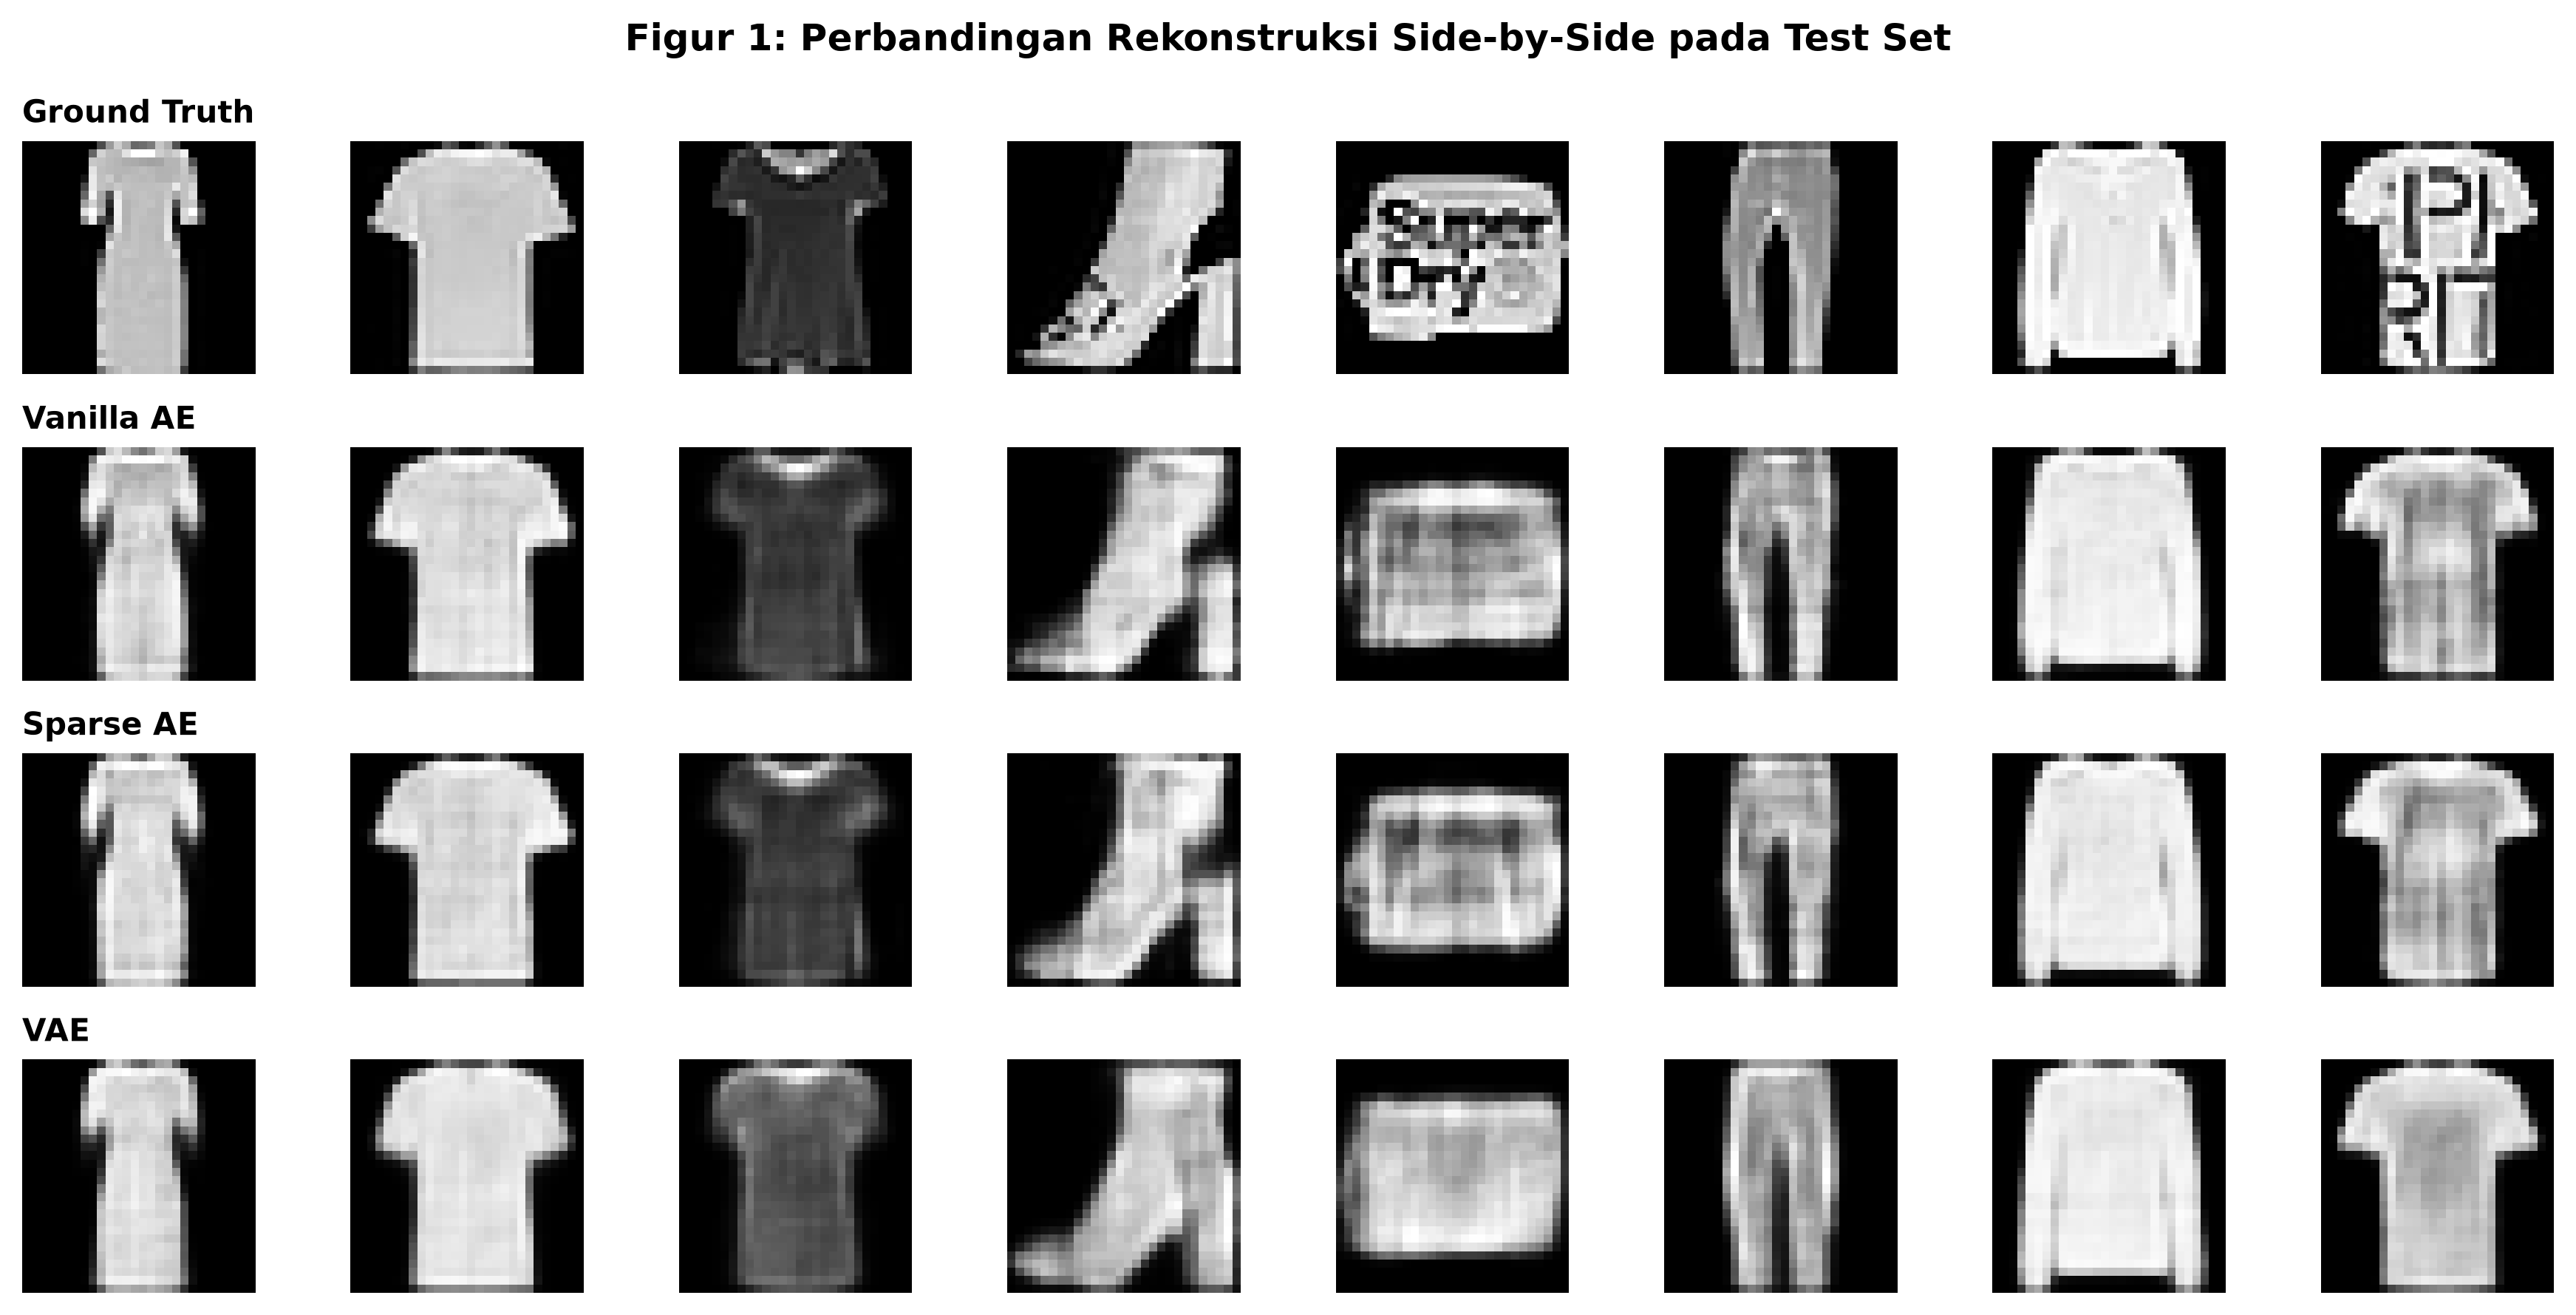
\includegraphics[width=0.94\textwidth]{outputs/figures/figur1_rekonstruksi.png}
  \caption{Perbandingan rekonstruksi 8 sampel Test Set antara Citra Asli (\textit{Ground Truth}), Vanilla AE, Sparse AE, dan VAE.}
  \label{fig:recon}
\end{figure}

\textbf{Analisis Visual Gambar~\ref{fig:recon}:} Vanilla AE dan Sparse AE mampu mempertahankan siluet makro serta pola kontras lokal (seperti motif strip tas, kerah baju, dan bentuk hak sepatu) secara sangat dekat dengan \textit{Ground Truth}, selaras dengan nilai SSIM keduanya yang hampir identik (0,7895 vs 0,7875). Penalti $L_1$ pada Sparse AE menekan aktivasi derau latar belakang tanpa merusak struktur tepi utama. Sebaliknya, rekonstruksi VAE terlihat jauh lebih buram (\textit{oversmoothed}) pada detail tekstur halus dan tepi objek (SSIM turun ke 0,6801) karena adanya tarikan regularisasi KL Divergence yang memaksa posterior setiap citra tumpang-tindih menuju prior $\mathcal{N}(0, I)$.

\subsection{Figur 2: Grid \textit{Random Generative Sampling} ($4 \times 4$)}
\begin{figure}[H]
  \centering
  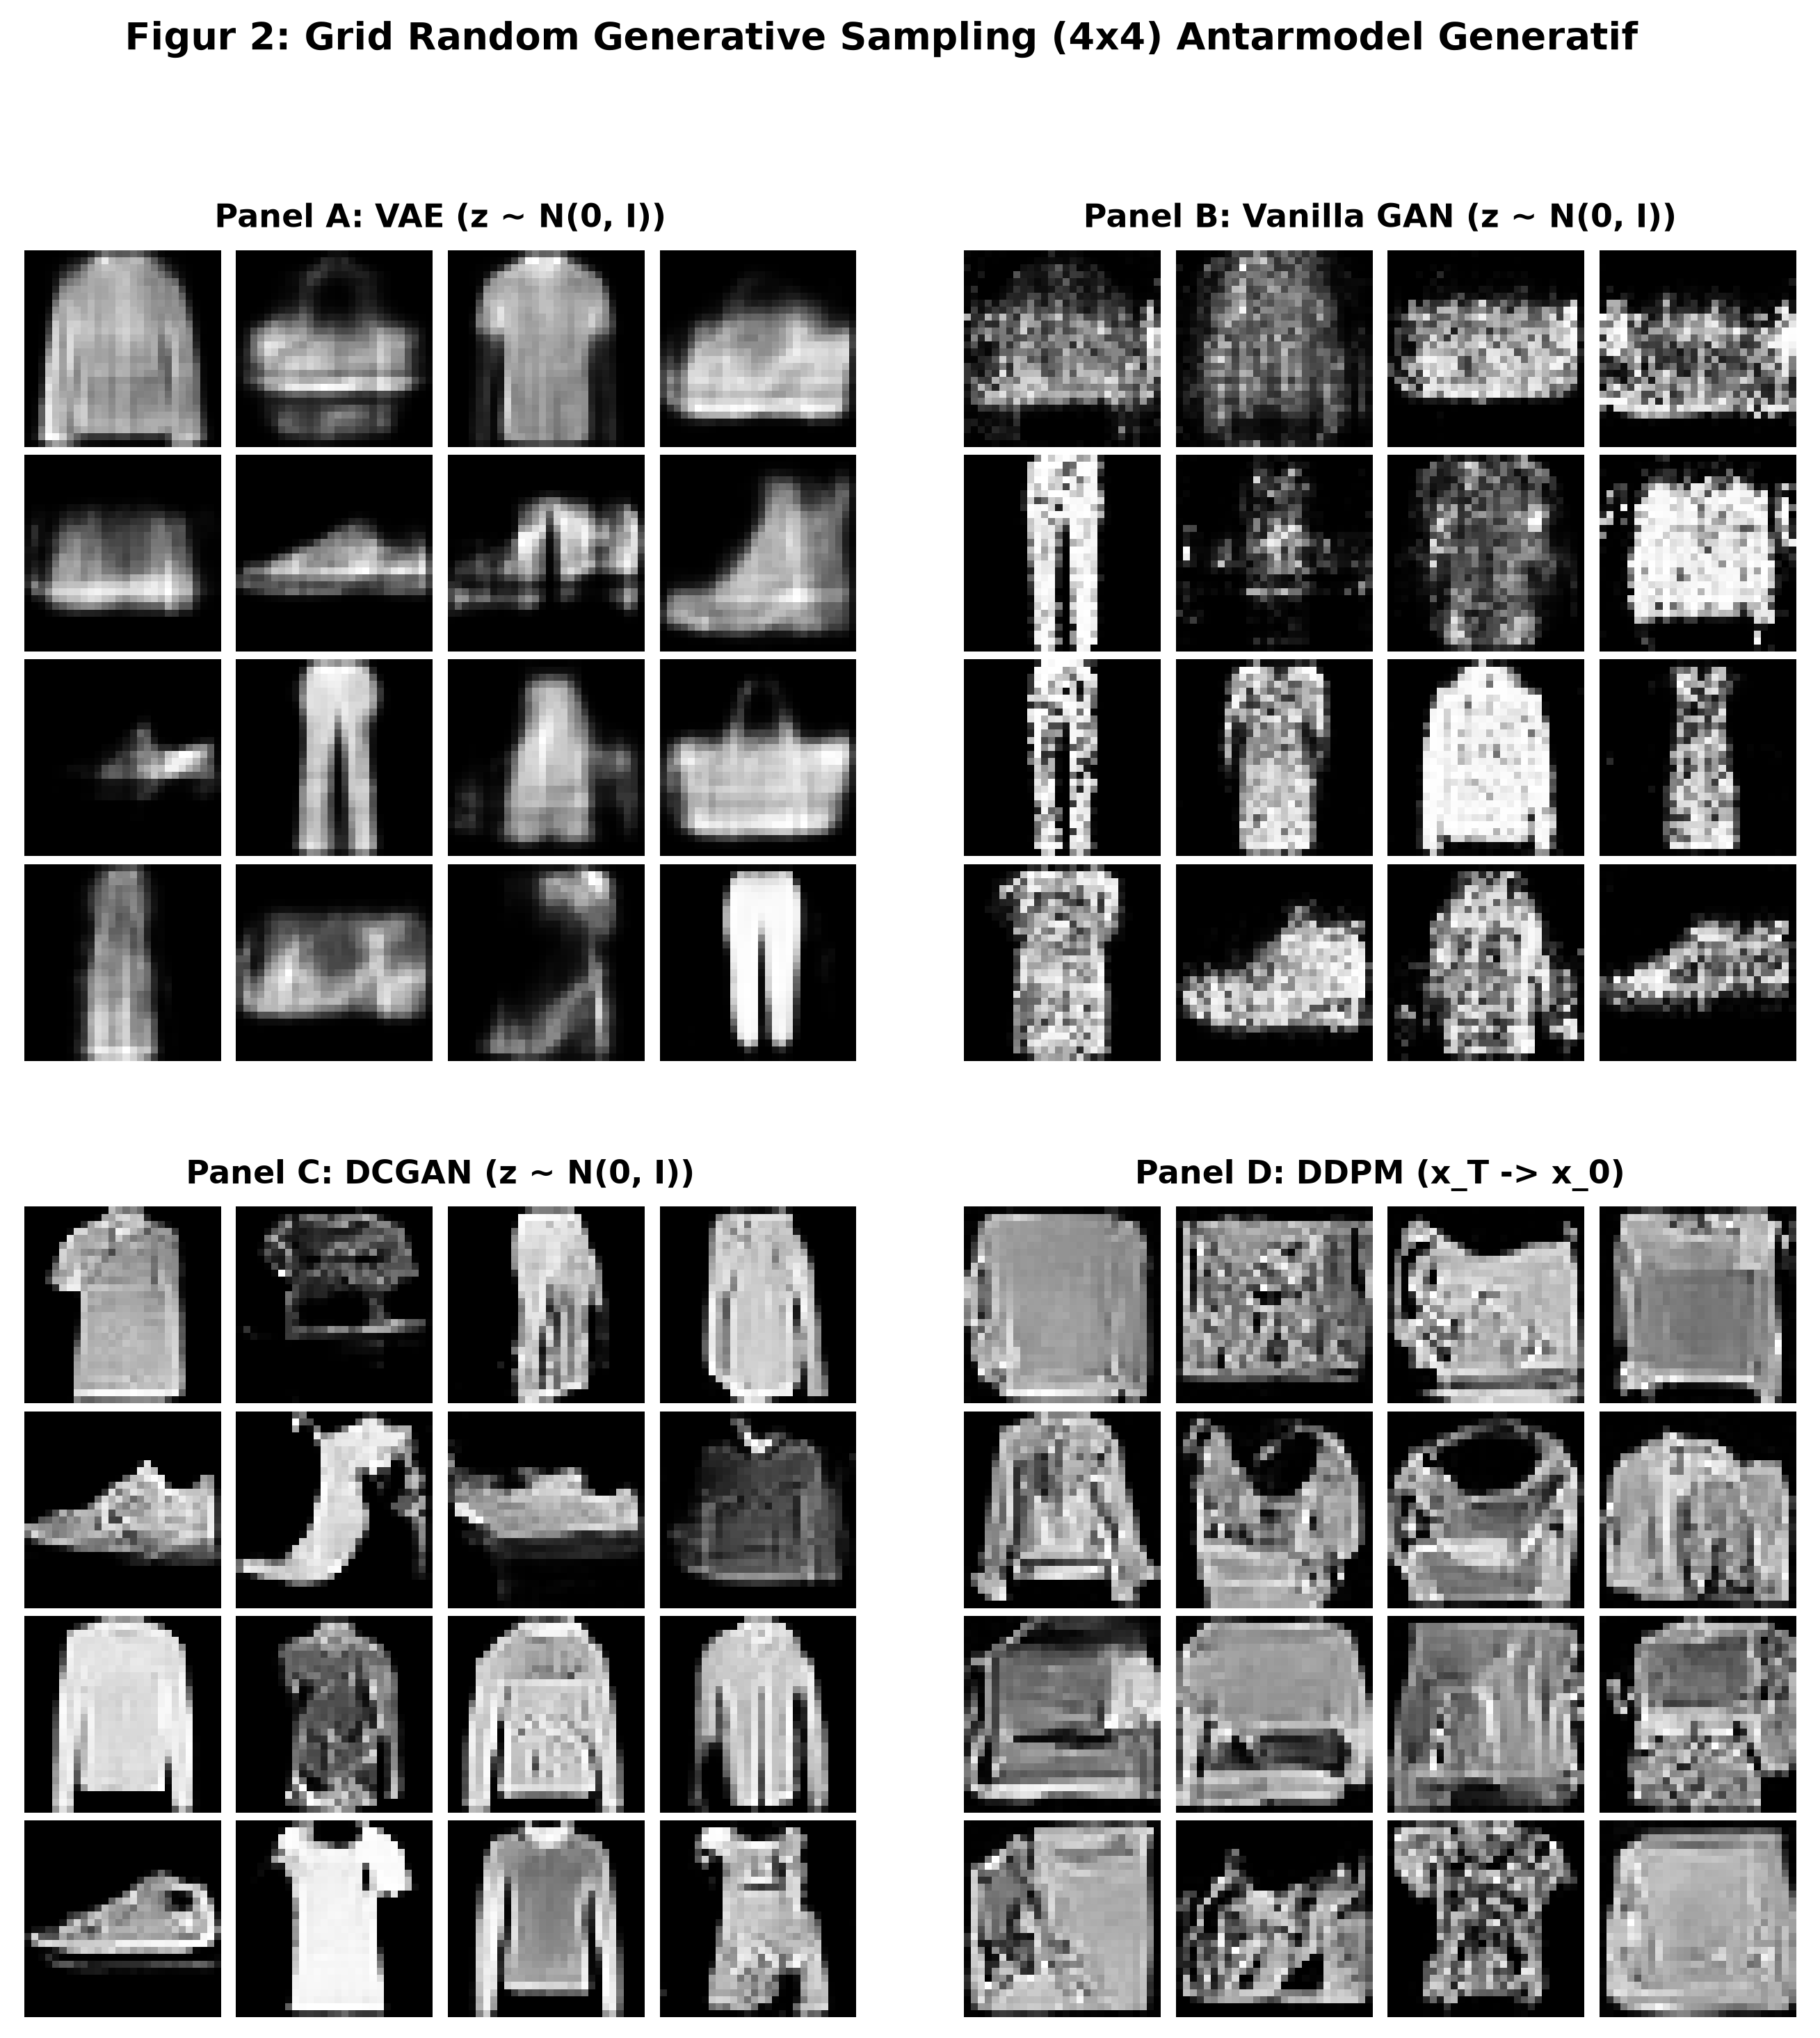
\includegraphics[width=0.80\textwidth]{outputs/figures/figur2_random_sampling.png}
  \caption{Kisi $4 \times 4$ (16 sampel sintetis acak) dari VAE, Vanilla GAN, DCGAN, dan DDPM pada Fashion-MNIST.}
  \label{fig:sampling}
\end{figure}

\textbf{Analisis Visual Gambar~\ref{fig:sampling}:} Kontras antar-paradigma tampak sangat jelas. Panel A (VAE, FID 94,12) menunjukkan keberagaman kelas yang baik namun seluruh objek tampak kabur seperti berkabut. Panel B (Vanilla GAN, FID 147,31) menampilkan kontur lebih kontras daripada VAE, tetapi mengandung derau piksel berbintik (\textit{salt-and-pepper artifacts}) serta bentuk objek yang terdistorsi akibat ketiadaan konektivitas spasial pada lapisan \textit{fully-connected}. Panel C (DCGAN, FID 29,10) menghasilkan siluet pakaian, sepatu, dan celana yang paling tajam, utuh, dan realistis secara struktural berkat operasi konvolusi transposisi. Panel D (DDPM, FID 91,54) menampilkan keberagaman mode (\textit{mode diversity}) tinggi dengan batas objek yang bersih, meskipun pada kapasitas Mini U-Net dan anggaran 25 epoch ($T=200$) sebagian tekstur halus belum seketat DCGAN.

\subsection{Figur 3: Bukti Empiris Batasan Bobot dan \textit{Latent Features} MLP Classifier}
\begin{figure}[H]
  \centering
  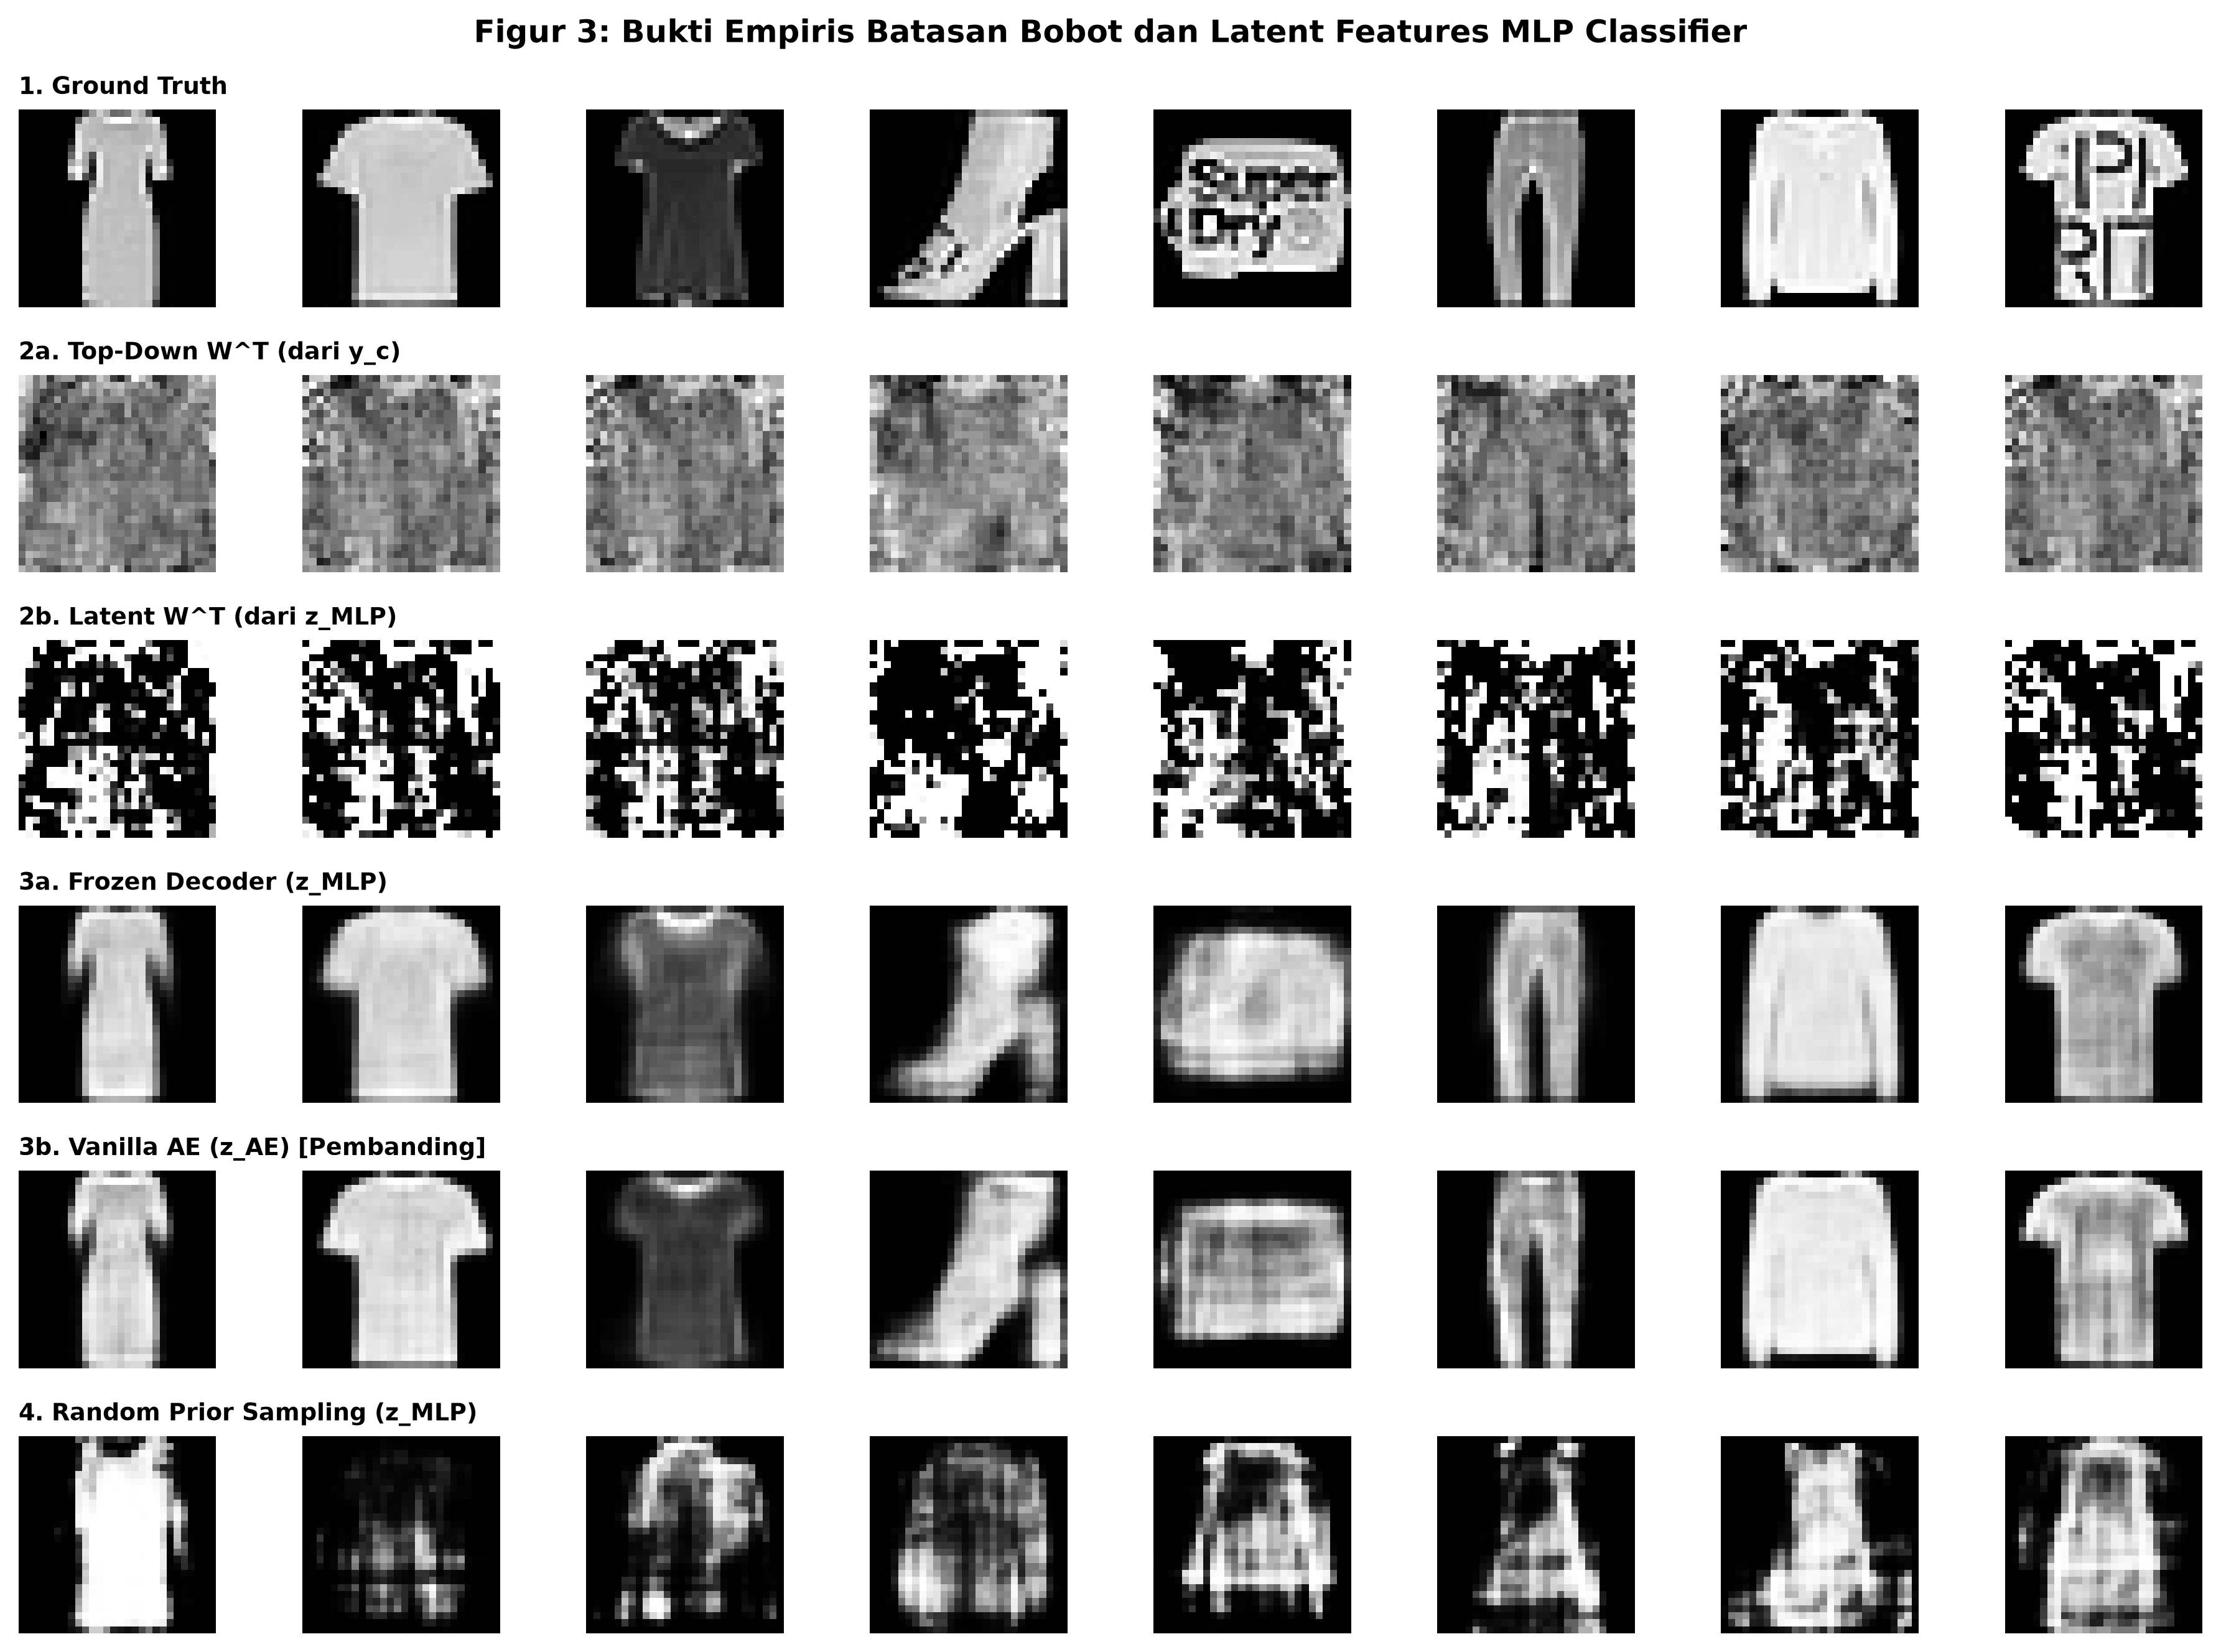
\includegraphics[width=0.90\textwidth]{outputs/figures/figur3_mlp_limitations.png}
  \caption{Perbandingan visual empat kelompok pembuktian empiris batasan MLP Classifier terhadap pembanding Vanilla AE.}
  \label{fig:mlp_limit}
\end{figure}

\textbf{Analisis Visual Gambar~\ref{fig:mlp_limit}:} Baris 2a (proyeksi balik transpos bobot $W^T$ dari $y_c$) dan Baris 2b (transpos dari $z_{\text{MLP}}$) gagal total menampilkan bentuk pakaian dan hanya membentuk pola bercak tekstur statis berulang, membuktikan $W^T \neq W^{-1}$. Pada Baris 3a, meski Frozen Latent Decoder telah dilatih khusus memakai MSE Loss, hasil rekonstruksinya tampak generik seperti ``rata-rata prototipe kelas'' dan kehilangan ciri spesifik individu citra (bandingkan ketajaman detailnya dengan Baris 3b Vanilla AE). Baris 4 memperlihatkan bahwa penarikan sampel acak $\mathcal{N}(\mu_z, \text{diag}(\sigma_z^2))$ pada ruang laten MLP menghasilkan bentuk kabur tak terdefinisi karena ketiadaan struktur manifold kontinu.

\subsection{Figur 4: \textit{Linear Latent Space Interpolation}}
\begin{figure}[H]
  \centering
  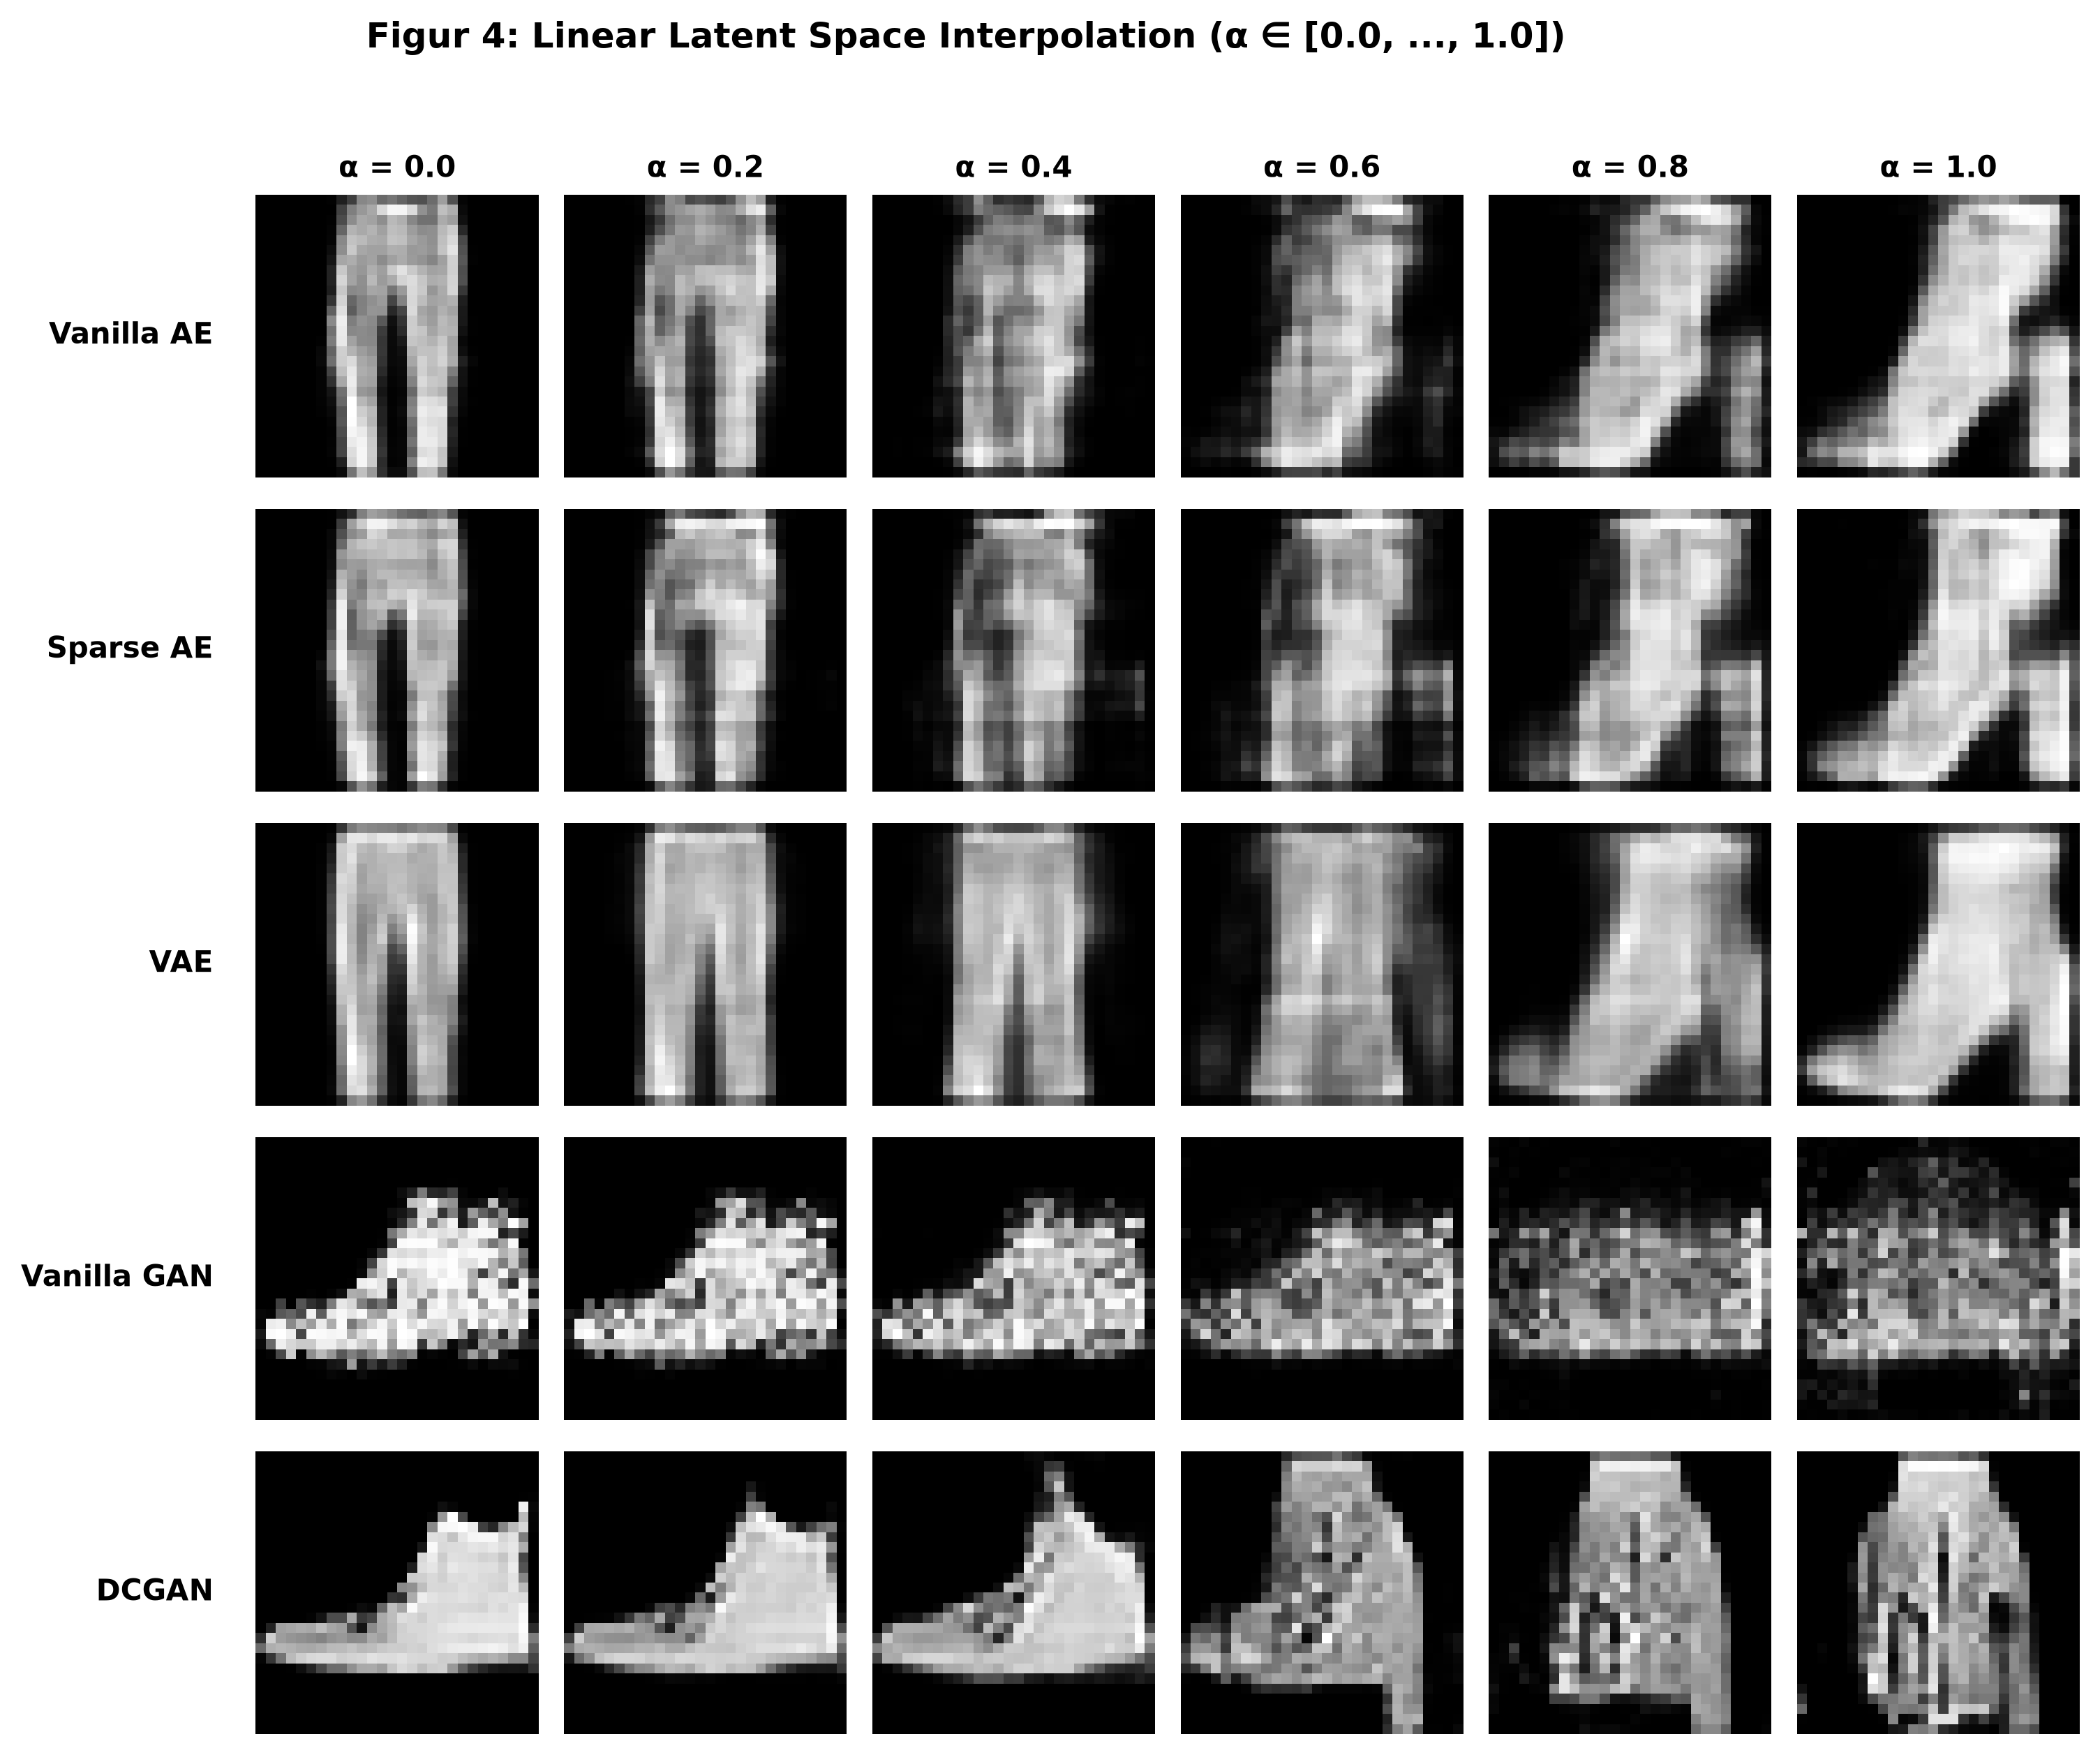
\includegraphics[width=0.86\textwidth]{outputs/figures/figur4_latent_interpolation.png}
  \caption{Interpolasi linier $z(\alpha) = (1-\alpha)z_A + \alpha z_B$ dengan $\alpha \in \{0.0, 0.2, 0.4, 0.6, 0.8, 1.0\}$ pada lima model generatif.}
  \label{fig:interp}
\end{figure}

\textbf{Analisis Visual Gambar~\ref{fig:interp}:} Pada transisi antara dua kelas kontras (celana panjang $\alpha=0,0$ menuju sepatu bot $\alpha=1,0$), Vanilla AE dan Sparse AE menunjukkan efek \textit{ghosting} (tumpang-tindih transparan dua gambar yang saling menimpa secara kasar pada $\alpha \in [0.4, 0.6]$) alih-alih transformasi geometris yang mulus. Fenomena ini terjadi karena lintasan garis lurus di ruang laten deterministik melintasi wilayah kosong (\textit{latent space voids}) yang belum pernah dilatih oleh dekoder. Sebaliknya, VAE, Vanilla GAN, dan terutama DCGAN memperlihatkan transisi morfologis yang kontinu dan teratur dari satu objek ke objek lain karena ruang laten ketiganya terpetakan padat terhadap distribusi prior Gaussian $\mathcal{N}(0, I)$.

\subsection{Figur 5: \textit{Training Loss Curves} dan \textit{DDPM Denoising Trajectory}}
\begin{figure}[H]
  \centering
  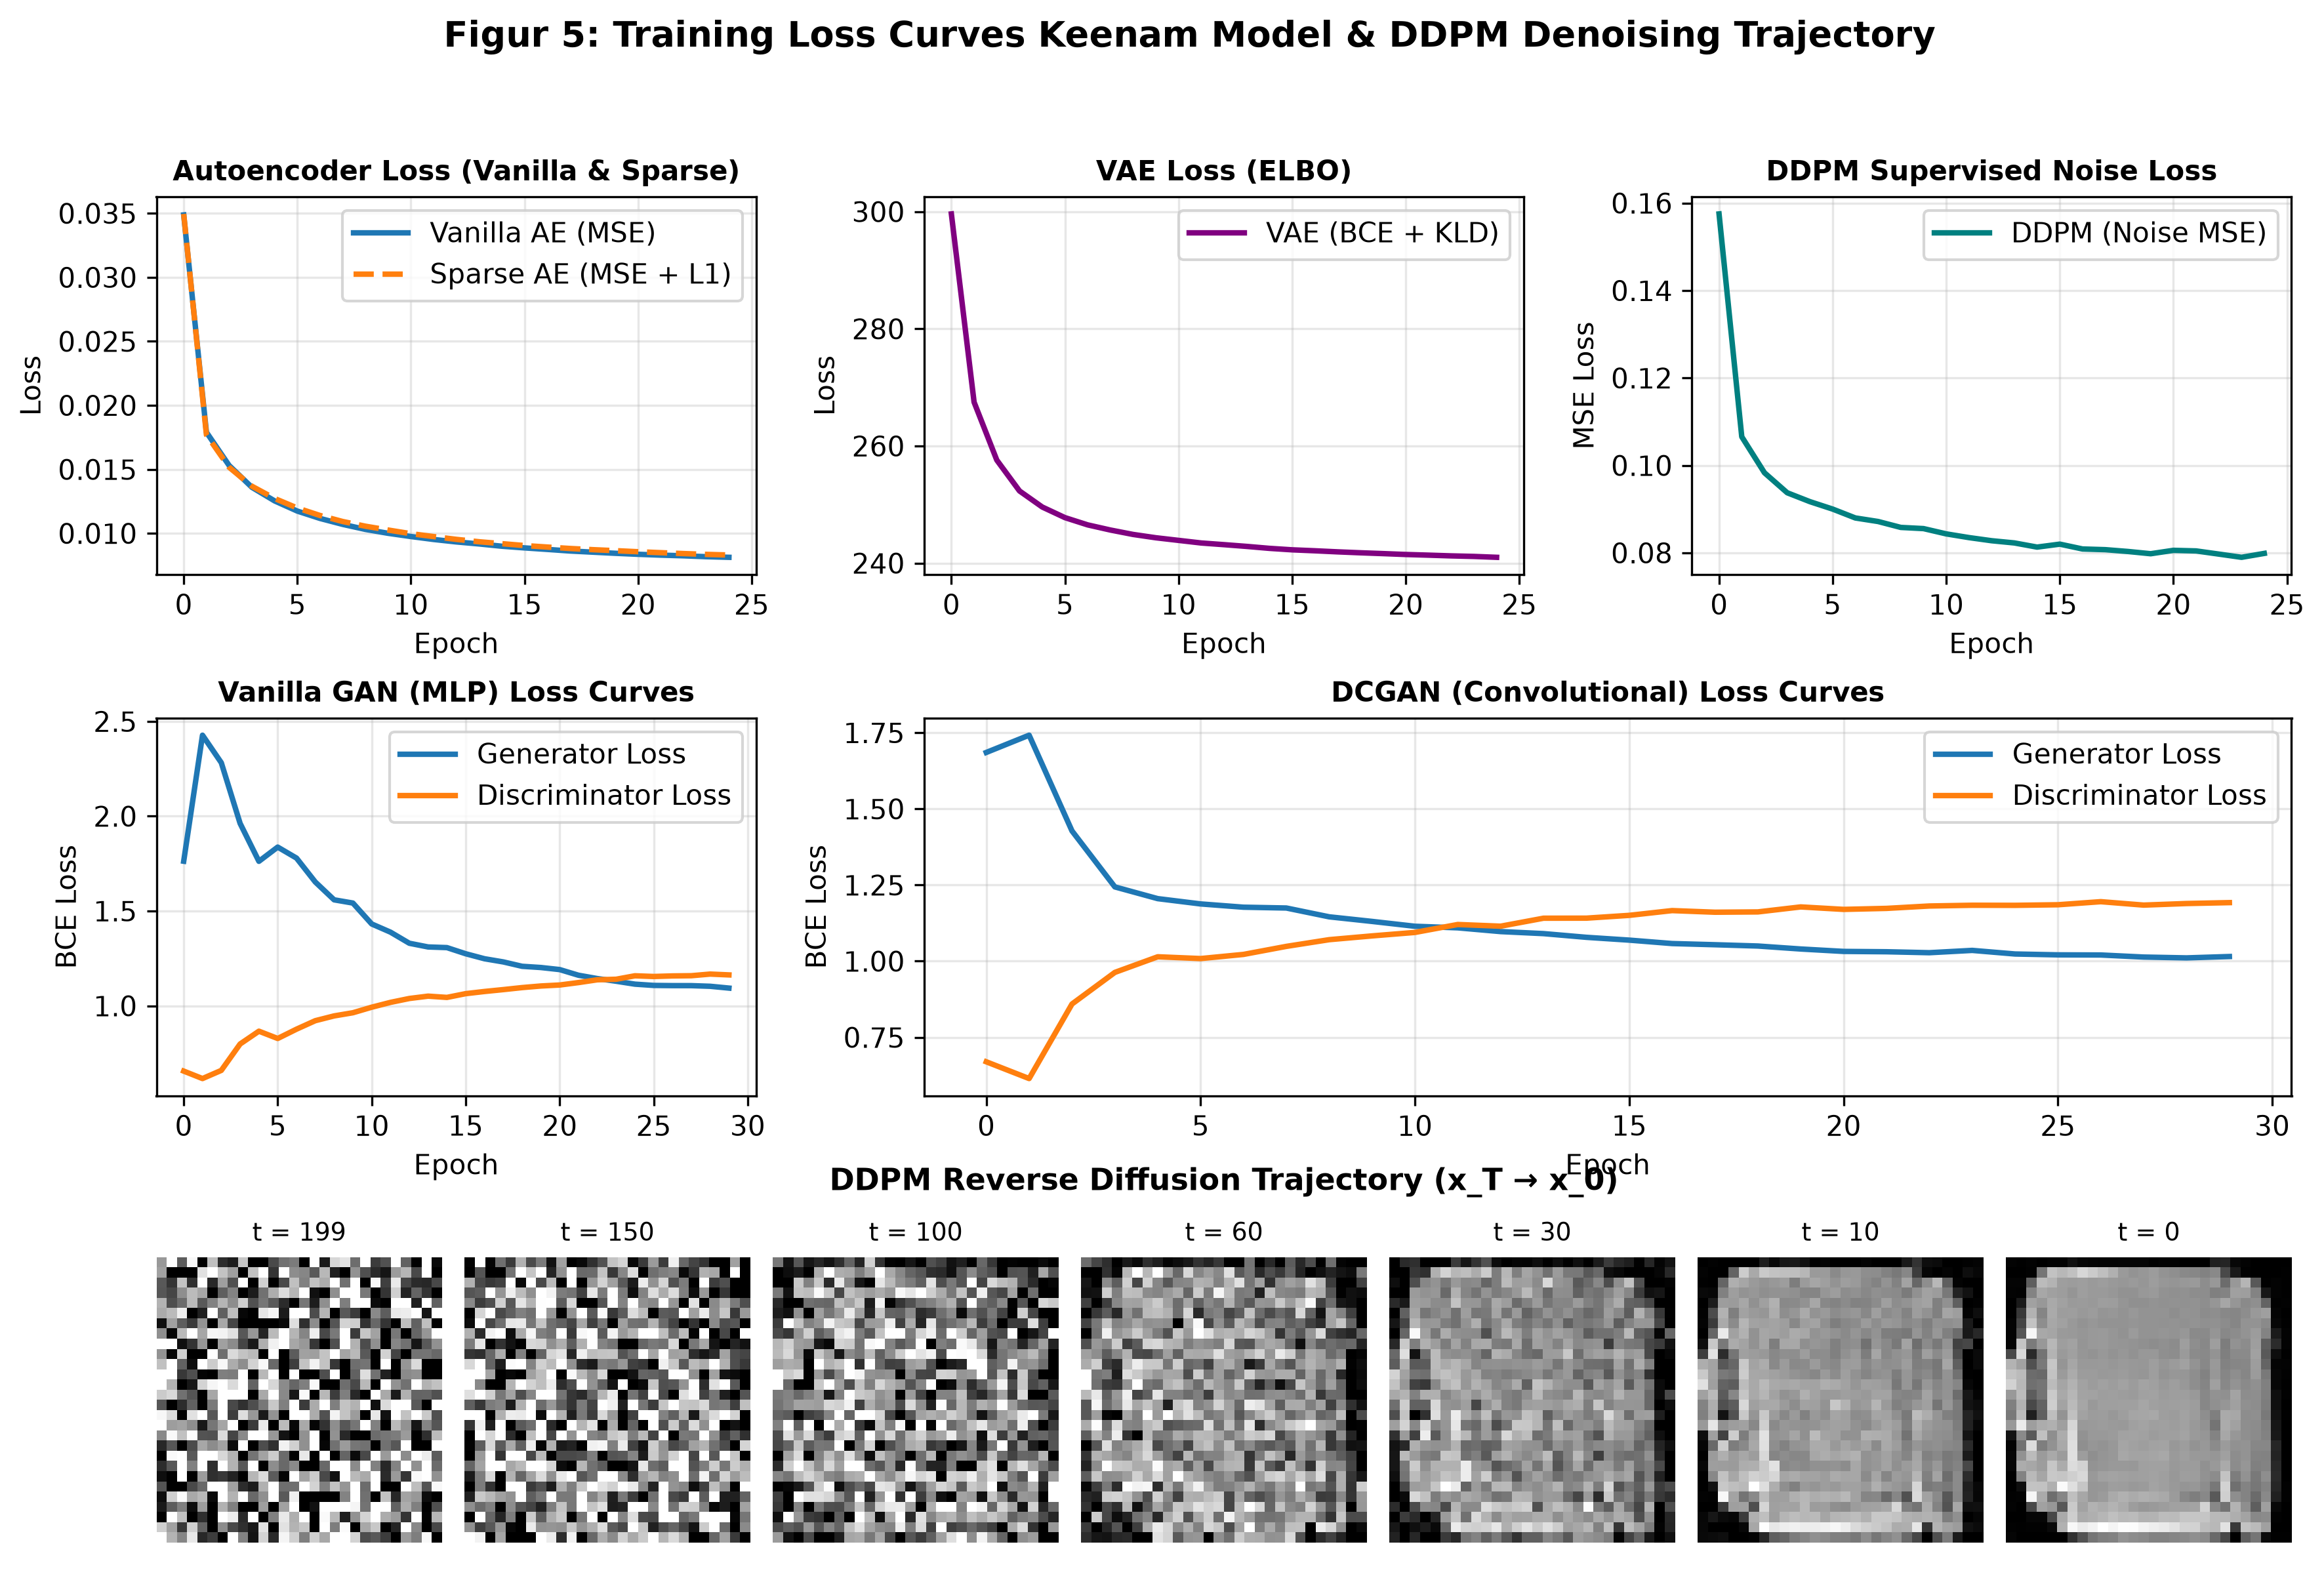
\includegraphics[width=0.95\textwidth]{outputs/figures/figur5_loss_and_trajectory.png}
  \caption{Kurva \textit{training loss} keenam model selama pelatihan serta sekuens \textit{reverse diffusion} DDPM ($x_T \rightarrow x_0$).}
  \label{fig:loss_traj}
\end{figure}

\textbf{Analisis Visual Gambar~\ref{fig:loss_traj}:} Berdasarkan catatan \texttt{loss\_history.json}, Vanilla AE ($0,03488 \rightarrow 0,00813$), Sparse AE ($0,03495 \rightarrow 0,00831$), VAE ($299,61 \rightarrow 241,00$), dan DDPM ($0,15752 \rightarrow 0,07988$, minimum $0,07898$ pada epoch 24) seluruhnya menunjukkan penurunan loss yang monoton dan konvergen stabil. Sebaliknya, pada panel GAN terlihat dinamika permainan \textit{minimax}: pada Vanilla GAN, \textit{Generator Loss} melonjak tajam hingga 2,427 pada epoch 2 saat \textit{Discriminator Loss} jatuh ke 0,616 sebelum perlahan menyeimbangkan diri (akhir G 1,093 vs D 1,163). DCGAN meredam lonjakan awal tersebut (puncak G hanya 1,742, lalu melandai stabil ke 1,015 vs D 1,192). Panel bawah memperlihatkan mekanisme kerja DDPM secara visual: dari derau Gaussian murni pada $t=199$, struktur global mulai terbentuk pada $t \in [60, 30]$, dan detail kontur pakaian mengeras tajam pada langkah akhir $t=10 \rightarrow t=0$.

% --------------------------------------------------------------------
% BAGIAN VI: PEMBAHASAN KRITIS, JAWABAN Q1-Q6, & REKOMENDASI INDUSTRI
% --------------------------------------------------------------------
\section{Pembahasan Kritis, Jawaban Pertanyaan Penelitian, dan Rekomendasi Industri}

\subsection{Q1: Perbandingan Kuantitatif \textit{Reconstruction Fidelity} vs \textit{Generative Quality}}
Pada dimensi fidelitas rekonstruksi (Tabel~\ref{tab:metrics}), \textbf{Vanilla AE} mencapai kinerja terbaik dengan Test MSE \textbf{0,00838}, PSNR \textbf{20,77 dB}, dan SSIM \textbf{0,7895}. Penambahan penalti kelangkaan $\lambda \|h\|_1$ ($\lambda = 10^{-4}$) pada \textbf{Sparse AE} hanya meningkatkan MSE secara marjinal sebesar \textbf{+0,72\%} menjadi \textbf{0,00844} (PSNR 20,74 dB; SSIM 0,7875). Selisih yang sangat kecil ini menunjukkan bahwa representasi jarang mampu mempertahankan hampir seluruh kapasitas rekonstruksi sembari menekan aktivasi neuron yang tidak esensial. Sebaliknya, \textbf{VAE} mengalami degradasi rekonstruksi signifikan dengan MSE melonjak \textbf{1,86$\times$} (+85,68\%) menjadi \textbf{0,01556}, PSNR turun \textbf{-2,69 dB} (18,08 dB), dan SSIM merosot menjadi \textbf{0,6801}. Penurunan ini adalah konsekuensi matematis langsung dari suku $D_{\text{KL}}(q(z|x)\,\|\,\mathcal{N}(0,I))$ dalam objektif ELBO yang membatasi kapasitas informasi (\textit{rate-distortion trade-off}) guna memaksa keteraturan ruang laten.

Sebaliknya, pada dimensi kualitas generatif dari prior acak $z \sim \mathcal{N}(0, I)$, Vanilla AE dan Sparse AE tidak dapat dievaluasi FID-nya secara valid karena ruang laten deterministiknya penuh \textit{voids}. Di antara keempat model generatif sejati, \textbf{DCGAN} memimpin jauh dengan skor FID \textbf{29,10}, diikuti \textbf{DDPM} (\textbf{91,54}), \textbf{VAE} (\textbf{94,12}), dan \textbf{Vanilla GAN} (\textbf{147,31}). Mengganti lapisan MLP pada Vanilla GAN menjadi arsitektur konvolusional penuh pada DCGAN memangkas skor FID sebesar \textbf{80,25\%} (5,06$\times$ lebih baik).

\subsection{Q2: Analisis \textit{Blurriness} vs \textit{Sharp Edges} dan Representasi Fitur}
Fenomena keburaman pada Vanilla AE, Sparse AE, dan terutama VAE berakar pada sifat matematis \textit{pixel-wise reconstruction loss} (MSE/BCE). Ketika distribusi kondisional sebenarnya $P(x|z)$ bersifat multimodal (misalnya beberapa variasi kontur lengan atau tekstur kain berkorespondensi pada wilayah laten berdekatan), minimisasi galat kuadrat $\mathbb{E}_{x \sim P(x|z)}[\|x - \hat{x}\|_2^2]$ memiliki solusi analitis optimal berupa \textbf{ekspektasi kondisional}:
\begin{equation}
  \hat{x}^* = \arg\min_{\hat{x}} \mathbb{E}_{x \sim P(x|z)}\left[\|x - \hat{x}\|_2^2\right] = \mathbb{E}[x|z]
\end{equation}
Karena rata-rata matematis dari beberapa mode citra tajam adalah superposisi piksel bernilai abu-abu menengah di sepanjang tepi objek, hasil prediksi $\hat{x}^*$ secara inheren menjadi buram (\textit{blurry}). Efek ini semakin parah pada VAE karena injeksi derau stokastik $z = \mu + \sigma \odot \epsilon$ memperlebar ketidakpastian pemetaan $z \mapsto x$.

Berbeda secara fundamental, \textit{adversarial loss} pada Vanilla GAN dan DCGAN tidak membandingkan piksel demi piksel, melainkan meminimalkan divergensi Jensen-Shannon $D_{\text{JS}}(P_{\text{data}} \| P_g)$ melalui jaringan Discriminator. Karena citra yang buram tidak pernah muncul pada distribusi data riil $P_{\text{data}}$, Discriminator akan menghukum keras setiap ketidakjelasan tepi sebagai sampel palsu ($D(\tilde{x}) \rightarrow 0$). Hal ini memaksa Generator memilih satu mode spesifik yang tajam pada setiap sampel $z$, menghasilkan kontur dan tekstur berfidelitas tinggi.

Sementara itu, perbandingan representasi tersembunyi antara Sparse AE dan Vanilla AE memperlihatkan perbedaan fungsi fitur: Vanilla AE cenderung mempelajari representasi padat (\textit{dense distributed coding}) yang tersebar merata pada seluruh 64 dimensi laten, sehingga rentan mendekati fungsi identitas jika kapasitas berlebih. Penalti $\lambda \|h\|_1$ pada Sparse AE mendorong mayoritas neuron laten menuju nol untuk setiap citra masukan, memaksa jaringan mempelajari kamus fitur lokal yang lebih selektif dan terdisentang (\textit{part-based localized features}) seperti tepi kerah, sol sepatu, atau siluet saku secara terpisah.

\subsection{Q3: Stabilitas Training, Dinamika Arsitektur, dan \textit{Generative Trilemma}}
Pada dinamika optimasi (Gambar~\ref{fig:loss_traj}), \textbf{Vanilla GAN} menunjukkan instabilitas khas permainan \textit{minimax}: pada awal pelatihan (epoch 2), Discriminator berbasis MLP terlalu cepat mendominasi ($D_{\text{loss}} = 0,616$) sehingga \textit{Generator Loss} melonjak hingga $2,427$. Dominasi Discriminator menyebabkan \textit{vanishing gradient} bagi Generator dan mendorong \textit{mode collapse} (Generator hanya mengulang sebagian kecil pola buram untuk mengecoh Discriminator), yang berujung pada FID terburuk (147,31). \textbf{DCGAN} memitigasi kendala ini secara drastis melalui empat prinsip arsitektur: (1) mengganti \textit{pooling} dan lapisan \textit{fully-connected} dengan \textit{strided/transposed convolution} yang membawa \textit{inductive bias} translasi spasial, (2) menerapkan \texttt{BatchNorm2d} untuk menstabilkan aliran gradien di seluruh lapisan (kecuali input D dan output G), (3) menggunakan aktivasi \texttt{LeakyReLU (0.2)} di Discriminator agar gradien negatif tidak mati, serta (4) inisialisasi bobot terstandarisasi $\mathcal{N}(0, 0.02)$. Hasilnya, kurva G dan D pada DCGAN bergerak lebih selaras dan menurunkan FID ke 29,10.

Membandingkan paradigma GAN dengan \textbf{DDPM}, terlihat keunggulan stabilitas optimasi yang kontras: GAN harus mencari titik pelana (\textit{saddle point} / Nash equilibrium) yang tidak pernah dijamin konvergen monoton, sedangkan DDPM memformulasikan pemodelan generatif sebagai masalah regresi \textit{supervised} sederhana (prediksi MSE atas derau $\epsilon$), sehingga kurva loss-nya turun mulus dari 0,1575 ke 0,0799 tanpa risiko \textit{mode collapse}.

Namun, hasil empiris ini secara tegas memverifikasi teori \textbf{Generative Trilemma} (\textit{Sample Quality}, \textit{Sampling Speed}, dan \textit{Mode Coverage}):
\begin{itemize}[leftmargin=1.4em, itemsep=2pt]
  \item \textbf{VAE (Cepat + Mode Coverage Tinggi, Kualitas Rendah):} Latensi \textit{single-pass} tercepat (\textbf{0,10 ms/batch 64}) dan mencakup seluruh mode data, tetapi kualitas sampel buram (FID 94,12).
  \item \textbf{DCGAN (Kualitas Tinggi + Cepat, Mode Coverage/Stabilitas Rentan):} Latensi \textit{single-pass} sangat cepat (\textbf{1,36 ms/batch 64} atau $\sim$0,021 ms/citra) dengan FID terbaik (\textbf{29,10}), tetapi sensitif terhadap arsitektur dan rawan menyempitkan variasi mode pada distribusi kompleks.
  \item \textbf{DDPM (Mode Coverage Tinggi + Stabil, Kecepatan Sangat Lambat):} Membutuhkan \textbf{727,22 ms/batch 64} (\textbf{534,7$\times$} lebih lambat dari DCGAN dan \textbf{7.272,2$\times$} lebih lambat dari VAE) karena harus melakukan 200 evaluasi berurutan jaringan Mini U-Net. Selain itu, eksperimen ini mengungkap catatan rekayasa penting: pada anggaran pelatihan terbatas (25 epoch, arsitektur ringan, $T=200$), DDPM belum mencapai potensi FID optimalnya (91,54) dibandingkan DCGAN (29,10), mengindikasikan bahwa keunggulan kualitas absolut DDPM membutuhkan kapasitas U-Net dan jadwal langkah difusi yang jauh lebih besar.
\end{itemize}

\subsection{Q4: Struktur \textit{Latent Space} dan Eksperimen Interpolasi}
Eksperimen interpolasi linier $z(\alpha) = (1-\alpha)z_A + \alpha z_B$ untuk $\alpha \in [0.0, 0.2, 0.4, 0.6, 0.8, 1.0]$ (Gambar~\ref{fig:interp}) memperlihatkan perbedaan struktur geometris ruang laten. Pada \textbf{Vanilla AE} dan \textbf{Sparse AE}, ketiadaan regularisasi prior membuat Encoder bebas memetakan setiap kelas ke pulau-pulau terpisah dalam $\mathbb{R}^{64}$ demi meminimalkan MSE semata. Ketika vektor interpolasi $z(\alpha)$ melintasi ruang di antara pulau-pulau tersebut (\textit{latent space voids}), Decoder dipaksa mengevaluasi titik di luar dukungan distribusi pelatihan (\textit{out-of-distribution}), sehingga memunculkan artefak visual rusak dan tumpang-tindih bayangan (\textit{ghosting}).

Sebaliknya, pada \textbf{VAE}, regularisasi KL Divergence memaksa seluruh distribusi posterior $q(z|x)$ saling berimpit dan mengisi bola kepadatan prior $\mathcal{N}(0, I)$ tanpa celah kosong. Akibatnya, setiap titik di sepanjang segmen garis $z(\alpha)$ tetap berada di dalam manifold laten kontinu yang terdefinisi baik, menghasilkan transisi semantik yang mulus antar-objek. Demikian pula pada \textbf{Vanilla GAN} dan \textbf{DCGAN}, karena Generator dilatih memetakan seluruh kepadatan prior kontinu $\mathcal{N}(0, I)$ langsung ke ruang citra, interpolasi antara dua vektor derau acak menghasilkan perubahan morfologis yang koheren dan tajam (terutama pada DCGAN).

\subsection{Q5: Pembuktian Ketidakmampuan Bobot dan Fitur Laten MLP Classifier}
Berdasarkan analisis Bagian~\ref{sec:mlp_proof} (Tabel~\ref{tab:mlp_vs_ae} dan Gambar~\ref{fig:mlp_limit}), kegagalan MLP Classifier (akurasi 88,61\%) dalam merekonstruksi maupun men-generate citra terbukti secara konsisten di ketiga sudut pandang matematis:
\begin{enumerate}[leftmargin=1.4em, itemsep=2pt]
  \item \textbf{Perspektif $P(y|x)$ dan \textit{Information Bottleneck}:} Cross-Entropy Loss membuang variasi intra-kelas yang tidak esensial untuk klasifikasi. Terbukti saat $z_{\text{MLP}}$ yang dibekukan di-decode ulang oleh jaringan MSE khusus, galat rekonstruksinya tetap 2,10$\times$ lebih buruk dari Vanilla AE (MSE 0,01758 vs 0,00838; PSNR turun 3,22 dB; SSIM turun 0,1339), hanya mampu menghasilkan rata-rata prototipe kelas yang kehilangan detail lokal.
  \item \textbf{Ketidakbalikan Bobot Non-Ortogonal ($W^T W \neq I$) \& ReLU:} Proyeksi balik langsung melalui transpos bobot $W^T$ baik dari $y_c$ maupun $z_{\text{MLP}}$ menghasilkan bercak abstrak tanpa struktur pakaian karena matriks persegi panjang terlatih tidak ortogonal dan operasi $\text{ReLU}(u) = \max(0, u)$ telah membuang seluruh aktivasi negatif secara permanen.
  \item \textbf{Absennya Regularisasi Prior $P(z)$:} Tanpa paksaan distribusi prior kontinu, penarikan sampel $z_{\text{rand}} \sim \mathcal{N}(\mu_z, \text{diag}(\sigma_z^2))$ gagal membentuk citra utuh karena mayoritas massa probabilitas Gaussian jatuh di luar klaster fitur kelas diskret MLP.
\end{enumerate}

\subsection{Q6: Sintesis Rekayasa dan Rekomendasi Industri}
Berdasarkan bukti empiris seluruh metrik (Tabel~\ref{tab:metrics}) dan karakteristik \textit{inductive bias} keenam model, rekomendasi arsitektur untuk tiga skenario deployment industri nyata dirangkum sebagai berikut:

\begin{enumerate}[leftmargin=1.4em, itemsep=3pt]
  \item \textbf{Deteksi Anomali Tanpa Supervisi pada Citra Inspeksi Manufaktur $\rightarrow$ Rekomendasi: \textit{Sparse Autoencoder}.}\\
  Meskipun Vanilla AE memiliki MSE uji sedikit lebih rendah (0,00838 vs 0,00844; selisih hanya 0,72\%), Vanilla AE rentan mempelajari fungsi identitas pada fitur berkapasitas besar sehingga berisiko ikut merekonstruksi cacat kecil (\textit{false negative}). Penalti $L_1$ pada Sparse AE memaksa jaringan mempelajari kamus fitur lokal yang ketat hanya untuk komponen produk normal. Saat citra cacat (goresan, retakan, atau komponen hilang) masuk, representasi jarang gagal memetakan pola anomali tersebut, menghasilkan lonjakan \textit{reconstruction error} lokal yang jauh lebih tajam dan diskriminatif untuk ambang batas deteksi anomali.

  \item \textbf{Filter Avatar Interaktif Waktu-Nyata pada Perangkat Mobile ($<30$ ms) $\rightarrow$ Rekomendasi: \textit{DCGAN}.}\\
  Dengan anggaran latensi ketat $<30$ ms, DDPM (727,22 ms/batch 64; $\sim$11,36 ms/citra di RTX 5070 dan dapat melonjak ratusan milidetik di NPU/CPU ponsel) langsung tereliminasi. Di antara model \textit{single-pass}, VAE memang tercepat (0,10 ms/batch 64), tetapi hasil visualnya buram (FID 94,12) sehingga tidak layak untuk aplikasi konsumen. Vanilla GAN (0,13 ms) juga gagal secara kualitas (FID 147,31, berbintik). \textbf{DCGAN} merupakan titik optimal: latensi batch 64 hanya \textbf{1,36 ms} ($\sim$0,021 ms/citra)---menyisakan margin sangat lega untuk perangkat mobile---sekaligus menghasilkan ketajaman visual terbaik (FID \textbf{29,10}) berkat struktur konvolusionalnya yang ramah akselerator mobile.

  \item \textbf{Pembuatan Aset Visual Beresolusi dan Berfidelitas Tinggi untuk Industri Kreatif $\rightarrow$ Rekomendasi: \textit{DDPM} (Skala Produksi) vs \textit{DCGAN} (Anggaran Komputasi Terbatas).}\\
  Untuk kebutuhan industri kreatif komersial yang tidak terkendala latensi \textit{real-time} (proses \textit{offline rendering}), \textbf{DDPM} (atau varian \textit{Latent Diffusion} modern) adalah pilihan strategis jangka panjang. Objektif prediksi derau yang sangat stabil (kurva loss turun mulus $0,1575 \rightarrow 0,0799$) menjamin \textit{mode coverage} penuh tanpa risiko \textit{mode collapse} saat diperbesar ke resolusi tinggi dan dataset multidomain yang sangat beragam, serta mudah dikondisikan dengan teks/kontrol spasial. Meski demikian, hasil empiris kita memberikan pelajaran rekayasa krusial: apabila anggaran komputasi dan jumlah epoch pelatihan sangat terbatas seperti pada studi ini (25 epoch, arsitektur ringan), \textbf{DCGAN} (FID 29,10) justru menghasilkan kualitas visual yang jauh lebih matang dan ekonomis dibanding DDPM (FID 91,54) dengan waktu pelatihan per epoch 39\% lebih singkat (9,21 s vs 15,17 s).
\end{enumerate}

\section{Kesimpulan}
Studi komparatif ini membuktikan bahwa pemilihan model generatif tidak dapat dipisahkan dari kausalitas matematis fungsi objektifnya. Model diskriminatif (MLP Classifier) secara fundamental tidak dapat menggantikan model generatif karena \textit{information bottleneck} $P(y|x)$, ketidakbalikan bobot $W^T \neq W^{-1}$, dan ketiadaan prior laten, yang terbukti menurunkan kualitas rekonstruksi hingga 2,10$\times$ lebih buruk dari Vanilla AE. Di antara enam keluarga model generatif pada Fashion-MNIST, Vanilla AE dan Sparse AE unggul mutlak pada rekonstruksi presisi (PSNR $\approx 20,7$ dB; SSIM $\approx 0,79$), VAE menyediakan manifold laten kontinu tercepat (0,10 ms) dengan kompromi keburaman, DCGAN meraih kualitas sampel sintetis terbaik (FID 29,10) dalam satu langkah cepat (1,36 ms), sementara DDPM menawarkan stabilitas optimasi dan cakupan mode tertinggi dengan konsekuensi latensi iteratif (727,22 ms) yang secara nyata mengonfirmasi hukum \textit{Generative Trilemma}.

\end{document}